%Se podrá presentar en dos Capítulos separados: Capítulo 4: Resultados y Capítulo 5: Discusión

%HIPÓTESIS: la linealidad se mantiene o no con la escala

\color{black} 
Con la intención de abarcar los dos bloques temáticos abordados en esta tesis, este capítulo se divide en dos partes. Inicialmente, se muestran los resultados obtenidos en cuanto al relevamiento de imágenes aéreas. A continuación, son presentados los resultados de los algoritmos de procesamiento.
\section {Propuesta de relevamiento por imágenes RGB de las reservas de la provincia de Misiones} \label{resultados bloque 1}


%% No olvidar mencionar que, por simplicidad en los cálculos se considera cada área como si fuera un cuadrado 
%%
En las tablas \ref{tab:yaboty}, \ref{tab:sanse} y \ref{tab:profundidad} se sumarizan los resultados del cálculo de tiempo de captura, costo y porcentaje de la imagen útil para cada tipo de plataforma analizada, habiéndose considerado 3 tipos de satélites, 2 tipos de aeronaves tripuladas y 3 modelos de VANT. Cada tabla para un tamaño de área relevada distinto. Como primer resultado destacable se puede observar de forma clara que para el caso de 20 hectáreas, el costo de obtención de las imágenes mediante VANT y aeronaves tripuladas es significativamente inferior al de las imágenes satelitales. Esto se debe fundamentalmente a que la adquisición de imágenes satelitales requiere de una superficie mínima, \SI{25}{\kilo\metre\squared} si las imágenes son de archivo (captura de más de 90 días) o de \SI{100}{\kilo\metre\squared} si son nuevas \cite{noauthor_satellite_2020}.

Por otro lado, el tiempo que lleva realizar la captura de imágenes que cubran toda el área a relevar depende de la plataforma que se use, y ese tiempo, además, se utilizó para la estimación del costo indicado en la tabla siguiendo lo detallado en la sección \ref{Metodo calculo relevamiento}. 

En el caso de los satélites el tiempo no es tenido en cuenta para el cálculo del costo, ni tampoco para la demora en su obtención, ya que se adquieren datos de archivo. En el caso de las aeronaves tripuladas y no tripuladas, tal como se mostró en la subsección \ref{Metodo calculo relevamiento}, el tiempo y el costo total dependerá de las características de los sensores (tamaño, distancia focal) y de las condiciones de sobrevuelo (altura sobre terreno, velocidad de desplazamiento). El costo total está estrechamente ligado al tiempo de relevamiento en el caso de aeronaves tripuladas o no, y para el caso de los satélites el costo proviene del prorrateo de costo de la misión y control del satélite, tomándose las tarifas comerciales.

Aún así, el porcentaje de utilidad de la imagen capturada se obtuvo dividiendo el tamaño de la reserva relevada por la superficie total relevada. En el caso de las imágenes satelitales, si el área relevada es menor a 2.500 hectáreas, a medida que el área de la reserva disminuya, también lo hará el porcentaje útil, como el área total de las imágenes es fija de 2.500 ha o \SI{25}{\kilo\metre\squared} porque es la mínima superficie que se puede adquirir. Para áreas más grandes, como el de la reserva Yaboty, el porcentaje útil será mayor, pero no puede precisarse \textit{a priori} sin conocer exactamente cuántas imágenes se necesitarán, ya que depende de la disponibilidad de las mismas según la trayectoria que tengan para el momento requerido. El costo total de captura de imágenes mediante vehículos aéreos tripulados o no, equipara e incluso supera al de imágenes satelitales. 

Adicionalmente se debe tener en cuenta la limitación de autonomía de VANT, que generalmente no superan la media hora \cite{noauthor_dji_nodate}, o la hora de autonomía en algunos casos \cite{noauthor_specs_nodate}, aunque hay algunos que llegan a dos horas de autonomía \cite{noauthor_us-1_nodate}. Esto indudablemente afecta al flujo de trabajo por la necesaria reposición de baterías, a la vez que deben establecerse numerosas bases operativas \footnote{Se entiende por base operativa el sitio desde el cual el VANT despega y aterriza por cada misión de relevamiento que realiza} en la medida en que se va avanzando con el relevamiento del terreno.

Otra limitación que se suma a los VANT es el alcance que tiene el mando de control. Los VANT comerciales más difundidos suelen tener alcances de hasta \SI{10}{\kilo\metre} \cite{noauthor_dji_nodate} por lo que esto debe ser tenido en cuenta en la extensión del área a relevar.

Por otro lado, en el caso de las aeronaves tripuladas pueden resultar muy inconvenientes en términos de erogación de dinero cuando se trata de pequeñas extensiones cuyo sobrevuelo de relevamiento es de relativa corta duración, mucho menor que media hora (ver tabla \ref{tab:avión}), ya que hay que sumar a toda la operatoria el traslado de la aeronave desde y hacia el aeródromo de base. Resulta evidente que será mayor la incidencia en el costo final la parte que corresponde al traslado en sí, si la superficie a ser relevada es de pocas hectáreas. En la provincia de Misiones existen en un radio menor a cincuenta kilómetros a las tres reservas analizadas algunos aeródromos o pistas que pueden usarse como base.


%\subsubsection{Cálculo presupuestario} %revisar si corresponde que quede aquí, en relación al párrafo precedente
Partiendo de las características del terreno a relevar (su extensión) y de la plataforma usada para la captura (dron con cámara/sensor) es posible acotar un marco presupuestario para llevar a cabo la tarea. Con los datos recabados, las estimaciones realizadas indican que para un relevamiento aéreo de un área de veinte hectáreas, es conveniente un VANT, ya que el costo total no excedería los 10 dólares, mientras que en un avión tripulado el costo total sería significativamente más alto, de alrededor de cinco o más veces, y una imagen satelital tendría un costo de 375 dólares (ver tabla \ref{tab:profundidad}. En el caso de un área un poco más grande, de cien hectáreas, el costo total con VANT sigue siendo más bajo que con las otras plataformas, con menos de 50 dólares, mientras que en un avión tripulado el costo total sería de por lo menos 53 dólares (ver tabla \ref{tab:sanse}), teniendo en cuenta que el aeródromo de base está situado a no más de quince minutos de vuelo. Finalmente para el caso de un área mucho más grande, de varios miles de hectáreas como la reserva Yaboty, se torna más conveniente el avión tripulado con alrededor de 20 mil dólares, un poco más que la mitad de lo que cuesta la imagen satelital, y muy por debajo del costo del VANT, que se aproxima o incluso supera el costo de las imágenes satelitales (ver tabla \ref{tab:yaboty}.

\begin{table}[]
    \begin{threeparttable}[b]
        \centering
        \caption{Tabla comparativa de tiempos y costos de relevamiento para la reserva Yaboty}
        \label{tab:yaboty}
        \begin{tabular}{ccccc}
            %\rowcolor[HTML]{C65911} 
            \hline 
            \hline 
            \multicolumn{2}{c}{\textbf{Yaboty}} &
              \multicolumn{3}{c}{\textbf{Superficie   250.000 ha}} \\
              \hline    
            %\rowcolor[HTML]{C65911} 
            \multicolumn{2}{c}{\textbf{Plataforma/modelo o tipo}} &
              \textbf{Tiempo {[}h{]}} &
              \textbf{Costo en USD \tnote{*}} &
              \textbf{Porcentaje útil de   imagen capturada} \\
              \hline 
              \hline 
             &
              { Pleiades} &
               &
              37.500,00 &
               \\
             &
              { Satellogic} &
               &
              37.500,00 &
               \\
            \multirow{-3}{*}{Satélite} &
              { IKONOS} &
              \multirow{-3}{*}{}{\tnote{**}} &
              37.500,00 &
              \multirow{-3}{*}{}{\tnote{***}} \\
             &
              { avión} &
              69,13 &
              16.590,65 &
              \textgreater{}90 \\
            \multirow{-2}{*}{Aeronave} &
              { helicóptero} &
              \multicolumn{2}{c} {s/d \tnote{****}}&
              \textgreater{}90 \\
             &
              { mavic   3m} &
              144,09 &
              28.098,33 &
              \textgreater{}90 \\
             &
              { asesor/9} &
              361,11 &
              70.416,36 &
              \textgreater{}90 \\
            \multirow{-3}{*}{VANT} &
              { mini 2} &
              314,23 &
              61.275,69 &
              \textgreater{}90 \\
             \hline
             \hline
        \end{tabular}
        \begin{tablenotes}
            \footnotesize{
            %\tiny{
           \item [*]Dólares estadounidenses.
           \item [**]El tiempo de captura de imágenes satelitales no se tiene en cuenta para el análisis de costo.
           \item [***]El porcentaje útil del área de la imagen no puede conocerse previamente, ya que depende de cuántas imágenes son necesarias para cubrir el área de interés, que a su vez dependen de la disponibilidad de las mismas.
           \item [****] sin datos
           }
         \end{tablenotes}
  \end{threeparttable}
\end{table}

%%%%%%%%%%%%%%%%%%%%%%%%%%%%%%%%%%%%%%%%%%%%%%%%%%%%%%%%%%%%%%%%%%%%%%%%%%%%%%%%%%%%%%%%%%%%%%%%%%%
% Please add the following required packages to your document preamble:
% \usepackage{multirow}
% \usepackage[table,xcdraw]{xcolor}
% Beamer presentation requires \usepackage{colortbl} instead of \usepackage[table,xcdraw]{xcolor}
\begin{table}[]
    \begin{threeparttable}[b]
        \centering
        \caption{Tabla comparativa de tiempos y costos de relevamiento para la reserva San Sebastián}
        \label{tab:sanse}
        \begin{tabular}{llclc}
            \hline
            \hline
            \multicolumn{2}{l}{\textbf{San Sebastián}}                                                                            & \multicolumn{3}{l}{\textbf{Superficie   100 ha}} \\ \hline
            \multicolumn{2}{l}{\cellcolor[HTML]{FFFFFF}\textbf{Plataforma/modelo o tipo}} &
              \multicolumn{1}{l}{\textbf{Tiempo {[}min{]}}} &
              
               \textbf{Costo en USD \tnote{*}}&
              \multicolumn{1}{l}{\textbf{Porcentaje útil de imagen capturada}} \\ \hline
            \cellcolor[HTML]{FFFFFF}                           & \cellcolor[HTML]{FFFFFF}{\color[HTML]{000000} Pleiades}   &          & 375,00 USD   & \multicolumn{1}{l}{}   \\
            \cellcolor[HTML]{FFFFFF}                           & \cellcolor[HTML]{FFFFFF}{\color[HTML]{000000} Satellogic} &  {\tnote{**}}  & 375,00 USD   & 4                   \\
            \multirow{-3}{*}{\cellcolor[HTML]{FFFFFF}Satélite} & \cellcolor[HTML]{FFFFFF}{\color[HTML]{000000} IKONOS}     &         & 375,00 USD   & \multicolumn{1}{l}{}   \\ \hline
            \cellcolor[HTML]{FFFFFF}                           & \cellcolor[HTML]{FFFFFF}{\color[HTML]{000000} avión}      & 42,24    &  53,74 USD 
 USD     & \textgreater{}90    \\
            \multirow{-2}{*}{\cellcolor[HTML]{FFFFFF}Aeronave} & {\color[HTML]{000000} helicóptero}                        & \multicolumn{2}{c}{s/d \tnote{***}} & \textgreater{}90    \\ \hline
                                                               & {\color[HTML]{000000} mavic   3m}                         & 5,12     & 16,63 USD    & \textgreater{}90    \\
                                                               & {\color[HTML]{000000} asesor/9}                           & 10,38    & 33,73 USD    & \textgreater{}90    \\
            \multirow{-3}{*}{VANT}                             & {\color[HTML]{000000} mini 2}                             & 9,34     & 30,37 USD    & \textgreater{}90    \\ \hline
            \hline
        \end{tabular}
        \begin{tablenotes}
            \footnotesize{
            %\tiny{
           \item [*]Dólares estadounidenses.
           \item [**]El tiempo de captura de imágenes satelitales no se tiene en cuenta para el análisis de costo.
           \item [***] sin datos
           }
         \end{tablenotes}
     \end{threeparttable}
\end{table}
%%%%%%%%%%%%%%%%%%%%%%%%%%%%%%%%%%%%%%%%%%%%%%%%%%%%%%%%%%%%%%%%%%%%%%%%%%%%%%%%%%%%%%%%%%%%%%%%%%%

% Please add the following required packages to your document preamble:
% \usepackage{multirow}
% \usepackage[table,xcdraw]{xcolor}
% Beamer presentation requires \usepackage{colortbl} instead of \usepackage[table,xcdraw]{xcolor}
\begin{table}[]
    \begin{threeparttable}[b]
        \centering
        \caption{Tabla comparativa de tiempos y costos de relevamiento para la reserva Profundidad}
        \label{tab:profundidad}
        \begin{tabular}{llclc}
            \hline
            \hline
            \multicolumn{2}{l}{\textbf{Profundidad}}                                                                            & \multicolumn{3}{l}{\textbf{Superficie   20 ha}} \\ \hline
            \multicolumn{2}{l}{\cellcolor[HTML]{FFFFFF}\textbf{Plataforma/modelo o tipo}} &
              \multicolumn{1}{l}{\textbf{Tiempo {[}min{]}}} &
              
               \textbf{Costo en USD \tnote{*}}&
              \multicolumn{1}{l}{\textbf{Porcentaje útil de imagen capturada}} \\ \hline
            \cellcolor[HTML]{FFFFFF}                           & \cellcolor[HTML]{FFFFFF}{\color[HTML]{000000} Pleiades}   &          & 375,00 USD   & \multicolumn{1}{l}{}   \\
            \cellcolor[HTML]{FFFFFF}                           & \cellcolor[HTML]{FFFFFF}{\color[HTML]{000000} Satellogic} &  {\tnote{**}}  & 375,00 USD   & 0,8                   \\
            \multirow{-3}{*}{\cellcolor[HTML]{FFFFFF}Satélite} & \cellcolor[HTML]{FFFFFF}{\color[HTML]{000000} IKONOS}     &         & 375,00 USD   & \multicolumn{1}{l}{}   \\ \hline
            \cellcolor[HTML]{FFFFFF}                           & \cellcolor[HTML]{FFFFFF}{\color[HTML]{000000} avión}      & 40,42  &  50,70 USD 
 USD     & \textgreater{}90    \\
            \multirow{-2}{*}{\cellcolor[HTML]{FFFFFF}Aeronave} & {\color[HTML]{000000} helicóptero}                        & \multicolumn{2}{c}{s/d \tnote{***}} & \textgreater{}90    \\ \hline
                                                               & {\color[HTML]{000000} mavic   3m}                         & 1,22     & 3,98 USD    & \textgreater{}90    \\
                                                               & {\color[HTML]{000000} asesor/9}                           & 2,19    & 7,13 USD    & \textgreater{}90    \\
            \multirow{-3}{*}{VANT}                             & {\color[HTML]{000000} mini 2}                             & 2,25     & 7,31 USD    & \textgreater{}90    \\ \hline
            \hline
        \end{tabular}
        \begin{tablenotes}
            \footnotesize{
            %\tiny{
           \item [*]Dólares estadounidenses.
           \item [**]El tiempo de captura de imágenes satelitales no se tiene en cuenta para el análisis de costo.
           \item [***] sin datos
           }
         \end{tablenotes}
     \end{threeparttable}
\end{table}

% Please add the following required packages to your document preamble:
% \usepackage[table,xcdraw]{xcolor}
% Beamer presentation requires \usepackage{colortbl} instead of \usepackage[table,xcdraw]{xcolor}
\begin{table}[]
    \begin{threeparttable}[b]
        \centering
        \caption{Tabla comparativa de tiempos de cada fase de operación de aeronave tripulada, estimados a partir de relevamientos y consultas hechas a personal del sector aeronáutico}
        \label{tab:avión}
        \begin{tabular}{lc}
            \hline
            \multicolumn{1}{c}{\textbf{Item}}   & \multicolumn{1}{l}{\textbf{Tiempo {[}min{]}}} \\ \hline
            \rowcolor[HTML]{FFFFFF} 
            Puesta en marcha, rodaje y despegue & 5                                             \\
            \rowcolor[HTML]{FFFFFF} 
            Traslado al área                    & 15                                            \\
            \rowcolor[HTML]{FFFFFF} 
            Relevamiento                        & {\color[HTML]{000000} \tnote{*}}                      \\
            \rowcolor[HTML]{FFFFFF} 
            Retorno al aeródromo de base        & {\color[HTML]{000000} 15}                     \\
            \rowcolor[HTML]{FFFFFF} 
            Aterrizaje, rodaje y apagado        & {\color[HTML]{000000} 5}                      \\ \hline
        \end{tabular}
         \begin{tablenotes}
            \footnotesize{
            %\tiny{
           \item [*]según requerimiento; en el caso de la reserva Yaboty son más de 69 horas.
                    }
         \end{tablenotes}
     \end{threeparttable}
\end{table}

%agregar gráfico final
\begin{figure}[h!]
    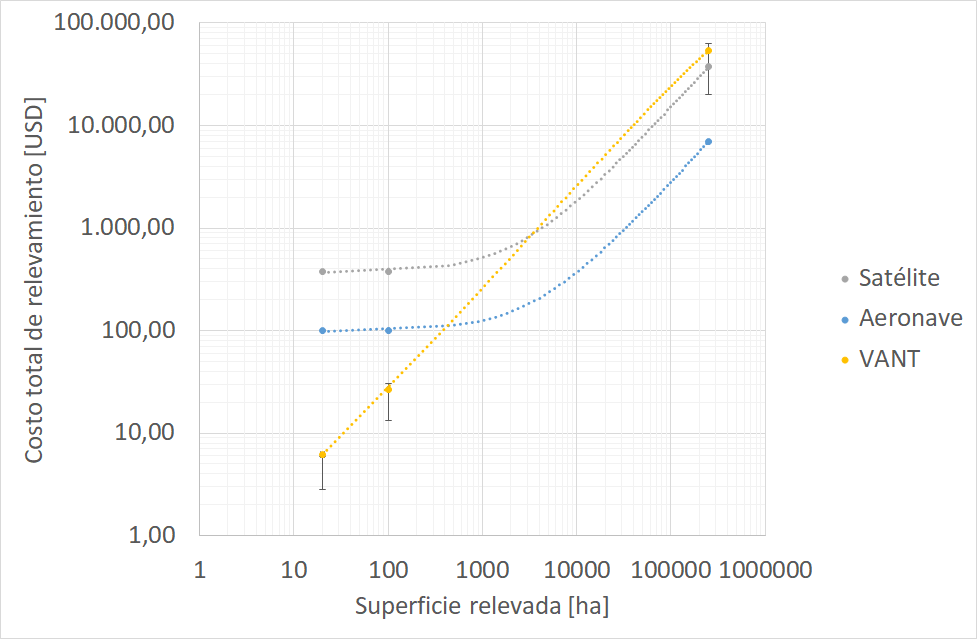
\includegraphics[width=\textwidth]{Imagenes/grafico bloque 1.png}
     \hfill
     \caption{Gráfico comparativo de costo total de relevamiento con distintas plataformas versus superficie relevada. Los costos se indican en dólares estadounidenses (USD)}
    \label{grafico_comparativo}
\end{figure}

\begin{figure}[h!]
    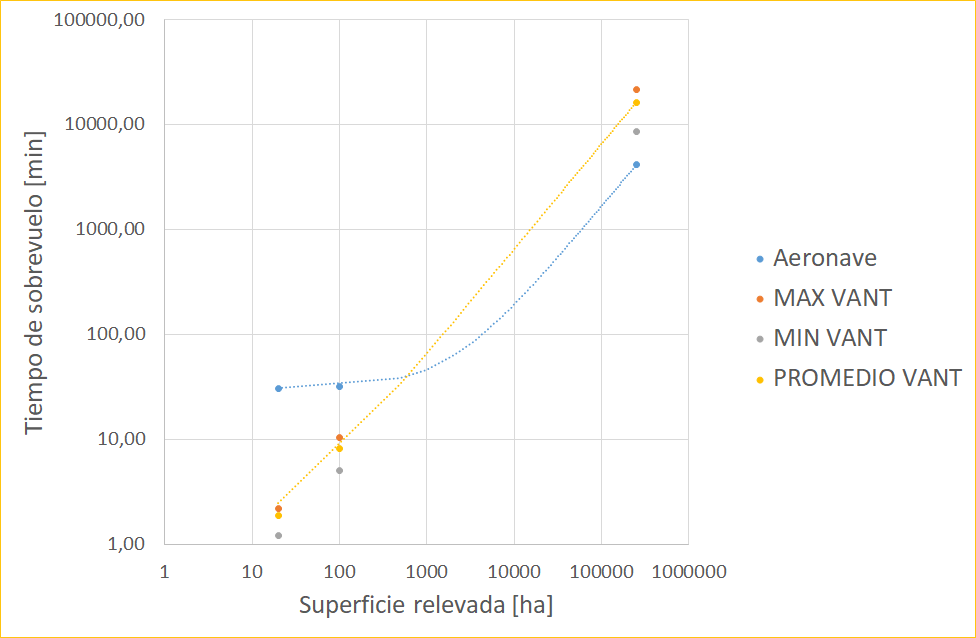
\includegraphics[width=\textwidth]{Imagenes/grafico bloque 1-II.png}
     \hfill
     \caption{Gráfico comparativo de tiempo total de relevamiento, incluyendo fase de despegue, desplazamiento y retorno a base, con distintas plataformas versus superficie relevada. Los costos se indican en dólares estadounidenses (USD)}
    \label{grafico_comparativo-II}
\end{figure}

En la figura \ref{grafico_comparativo} se muestra un gráfico en el que se expone cómo varía el costo de relevamiento expresado en dólares estadounidenses en relación al área relevada, expresada en hectáreas, según la plataforma usada, VANT, aeronaves tripuladas o satélites. Como se observa, en el caso de los VANT es claramente inferior el costo cuando se trata de superficies menores a mil hectáreas. A partir de ese valor el costo de relevamiento se asemeja al de la obtención de imágenes satelitales. Es marcada la incidencia que tiene en el caso de áreas relativamente pequeñas, de 100 hectáreas o menos, lo que puede definirse como costo fijo tanto para imágenes satelitales cuya adquisición está supeditada a un área no menor a \SI{25}{\kilo\metre\squared} (2.500 ha). De acuerdo con la figura \ref{grafico_comparativo} resulta evidente la conveniencia del uso de VANT en términos económicos para relevar las pequeñas reservas públicas y privadas en la provincia de Misiones.

De manera similar, en la figura \ref{grafico_comparativo-II} se muestra cómo varía el tiempo necesario para el relevamiento según la superficie y la plataforma usada. Según se aprecia, para áreas de pequeña extensión, de cien hectáreas o menos, el tiempo que demanda hacer el relevamiento con aeronave tripulada es de dos minutos o menos, con lo que el tiempo de relevamiento es insignificante en comparación al tiempo que podría definirse como logístico, desde la puesta en marcha, despegue, traslado y posterior retorno, que según muestra la tabla \ref{tab:avión}, se aproxima a la media hora. Ese tiempo es independiente de la superficie relevada, pero incide en el costo total, ya que es facturado en un servicio aéreo. Por otro lado, con el relevamiento con VANT se observa que para extensiones menores a 800 ha, es conveniente en términos de tiempo demandado en el relevamiento, incluso considerando el tiempo de reabastecimiento de la batería.

\subsection{Discusión}
De los resultados del análisis comparativo de las diferentes plataformas para obtención de las imágenes, se puede concluir que no hay una opción que de manera contundente sea superior y ventajosa respecto de las demás, sino que su elección dependerá del contexto, esencialmente la extensión del área a ser relevada. Como se ha visto, las imágenes satelitales presentan su ventaja en grandes extensiones (de más de 1000 ha), cuando los requerimientos de resolución espacial no son elevados, y si la disponibilidad temporal no presenta un condicionante. Para las extensiones relativamente pequeñas o medianas (menores a 1000 ha) las imágenes capturadas con VANT resultan ventajosas en cuanto a costos. La resolución espacial es también otro punto a favor.
\section{Resultados de los algoritmos de procesamiento de imágenes}
%\subsection{RESULTADOS Relación de iluminación natural con histogramas de color}
%Con el objeto de evaluar la correspondiente afectación en el histograma de las imágenes capturadas respecto a las condiciones de iluminación natural, se hicieron varias capturas en distintos horarios durante varios días desde una posición fija a un determinado objeto (un árbol de palta) y se midió la iluminancia usando un luxómetro.
%\color{cyan} %color de texto con 70-80 % o más de avance
\subsection{Análisis de regiones sombreadas mediante procesamiento homomórfico} \label{resultados homo}
Con el objetivo de lograr el análisis de forma automática de las imágenes RGB y pueda detectar estructura en la selva, tales como ejemplares altos y depresiones en el dosel de selva, se propone un algoritmo basado en la detección de sombras que se proyectan en el dosel. En esta sección se presentan los resultados del algoritmo basado en el análisis homomórfico cuyo detalle se desarrolló en la sección \ref{metod_homo_ventana} aplicados a una variedad de imágenes de la selva seleccionados. Las imágenes pueden verse en el anexo \ref{anexo_homo}.\\

Las primeras etapas del procesamiento según lo indicado en la figura \ref{flowchart_homomorfico} corresponden a cálculos matemáticos.
\subsubsection{Detección automática de regiones sombreadas mediante ventana deslizante} \label{resultados homo ventana}
El primer parámetro que se analiza es el tamaño de la ventana de exploración. Esta ventana es una región rectangular de la imagen definida en píxeles, la cual se va posicionando sobre la imagen analizada desplazándose gradualmente de izquierda a derecha y de arriba hacia abajo.
% Please add the following required packages to your document preamble:
% \usepackage{multirow}
\begin{table}[]
    \centering
    \begin{threeparttable}[b]
        
        \caption{Número de regiones sombreadas obtenidas por conteo manual y por el algoritmo automático de procesamiento homomórfico, como función del tamaño de ventana de exploración}
        % Please add the following required packages to your document preamble:
        \label{tab:resultados_homomorfico}
        \begin{tabular}{ccccccc}
        \hline
        \hline
                  & \textbf{Conteo}  & \multicolumn{5}{c}{\textbf{Tamaño de ventana [píxeles]}}   \\
            \textbf{Imagen}& \textbf{manual}  & \textbf{10 x 10}     & \textbf{15 x 15}     & \textbf{20 x 20 }   & \textbf{25 x 25}    & \textbf{30 x 30 }   \\ \hline
            \textbf{Par1d}  & 5  & 16      & 8      & 3     & 1     & 0     \\
            \textbf{Par2d}  & 2  & 11      & 4      & 2     & 0     & 0     \\
            \textbf{PNI1}   & 14 & 84     & 49     & 31    & 16    & 10    \\
            \textbf{PNI2}   & 14 & 67     & 50     & 20    & 13    & 6     \\
            \textbf{PNI3}   & 32 & 110    & 73     & 48    & 29    & 9     \\
            \textbf{PS1}    & 6  & 24     & 11     & 5     & 2     & 2     \\ 
            \textbf{YB1}    & 10 & 10     & 5      & 3     & 1     & 1     \\
            \textbf{YB2}    & 9  & 14     & 8      & 4     & 0     & 0     \\
            \textbf{ST1}    & 18 & 40     & 25     & 16    & 7     & 6     \\
            \textbf{ST2}    & 9  & 42     & 30     & 18    & 9     & 7     \\ \hline
            $e_{m}$\tnote{*}    & -  & -30,27 & -14,91 & -2,73 & 5,09  & 9,09  \\ 
            $\sigma^2_{e}$ \tnote{**}   & -  & 635,65  & 246,45 & 60,38 & 24,81 & 48,99 \\
           $\sigma_{e}$ \tnote{***}   & -  & 25,21  & 15,70  & 7,77  & 4,98  & 7,00 \\ \hline \hline
        \end{tabular}
        \begin{tablenotes}
        \footnotesize{
                \item [*]Error medio, obtenido mediante la fórmula $e_{m}=\frac{\Sigma(x_{m}-x_i)}{N}$
                \item [**]Varianza.
                \item [***] Desvío estándar.
                }
        \end{tablenotes}
  \end{threeparttable}
\end{table}
       
 Los resultados, que se exponen en la tabla \ref{tab:resultados_homomorfico} se analizan como función del tamaño de ventana de exploración.
Allí se visualiza para un total de once diferentes imágenes analizadas la cantidad de sombras detectadas, y se comparan los resultados de conteo automático con distintos tamaños de ventana, con el método de búsqueda de forma manual.

Se comprobó que eligiendo un tamaño de ventana de exploración igual a 20 por 20 píxeles se obtenía un acercamiento al criterio de selección manual.

Nótese el cambio de signo para el error medio entre los tamaños de ventana de 25 y de 20 píxeles por lado, indicando que la selección de un tamaño de ventana menor resultará en una mayor cantidad de sombras detectadas que la que se obtiene por conteo manual. En cambio un tamaño de ventana mayor podría obviar varias sombras que serían tenidas en cuenta para el conteo manual. De acuerdo con la resolución de las imágenes de prueba, el tamaño de ventana cuadrada de 20 píxeles por lado se correspondería con un área aproximada de \SI{100}{\metre\squared} , que bien podría corresponder a una copa de árbol de un diámetro aproximado de \SI{10}{\metre}.

%100 \SI{100}{\metre\squared}
El siguiente parámetro que se analizó es el umbral para la binarización (ver figura \ref{flowchart_homomorfico}), definiendo un valor que correspondía a una intensidad de cada píxel por encima del cual se consideraba como sombra. En este caso el valor de intensidad fue de 0,75 en valores de intensidad de píxeles normalizados, de acuerdo con varias pruebas realizadas en las imágenes analizadas.

Para la selección de sombras binarizadas se recorrió la matriz de la imagen con una ventana de inspección que abarcaba 25 píxeles por lado, de modo que se evaluó un conjunto de 625 píxeles. Luego de varias pruebas con diferentes imágenes, se estableció un umbral de 0,45 (45\%) para clasificar las sombras, de modo que los recintos de píxeles blancos que superaban ese umbral eran catalogados como sombras de árboles grandes.

A los efectos de mostrar el funcionamiento del algoritmo de búsqueda y conteo de sombras, se expone la figura \ref{sombratorogris}, en la que se visualiza la imagen satelital en escala de grises de una porción de la reserva privada Sombra de Toro, luego la imagen de salida del filtro homomórfico (figura \ref{ST filtro}), la imagen binarizada luego del filtrado homomórfico en la figura \ref{mascaraST} y las sombras seleccionadas con el algoritmo en la figura \ref{seleccionadaST}. En la figura \ref{ST25} se muestra



\begin{figure}[h!]
    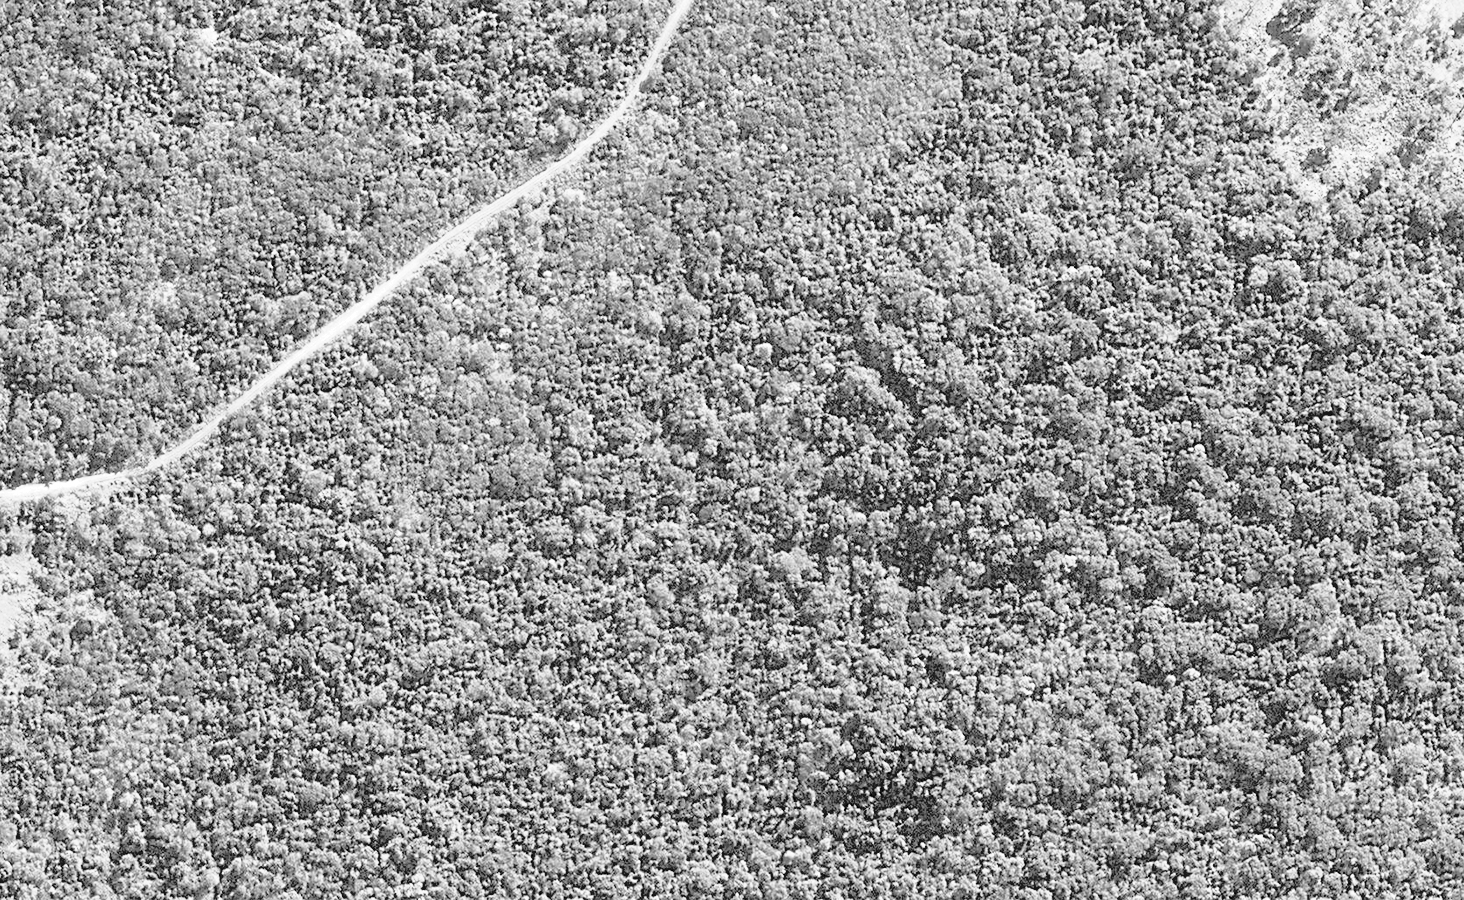
\includegraphics[width=\textwidth]{Imagenes/Homomorfico/ST2.png}
     \hfill
     \caption{Imagen aérea (satelital) de reserva privada Sombra de Toro (identificada como ST2 en la tabla), en escala de grises. Resolución de imagen de 1464 x 900 píxeles, resolución espacial de 0,5 m por pixel.}
    \label{sombratorogris}
\end{figure}

\begin{figure}[h!]
    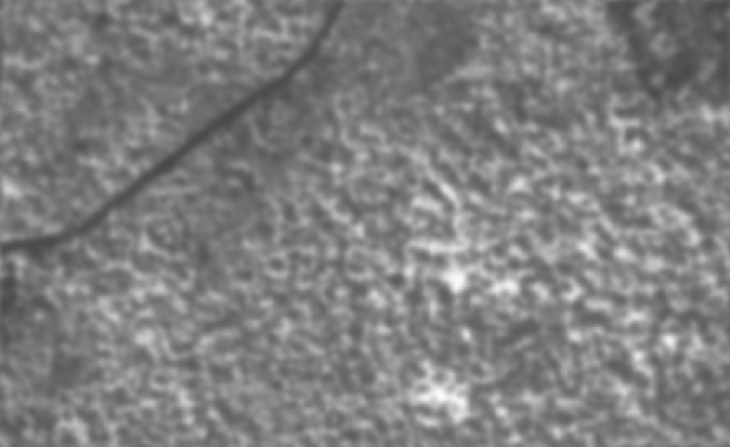
\includegraphics[width=\textwidth]{Imagenes/Homomorfico/ST2_filtro.png}
     \hfill
     \caption{Imagen filtrada aplicando el filtro homomórfico a la imagen de la figura \ref{sombratorogris}.}
    \label{ST filtro}
\end{figure}

\begin{figure}[h!]
    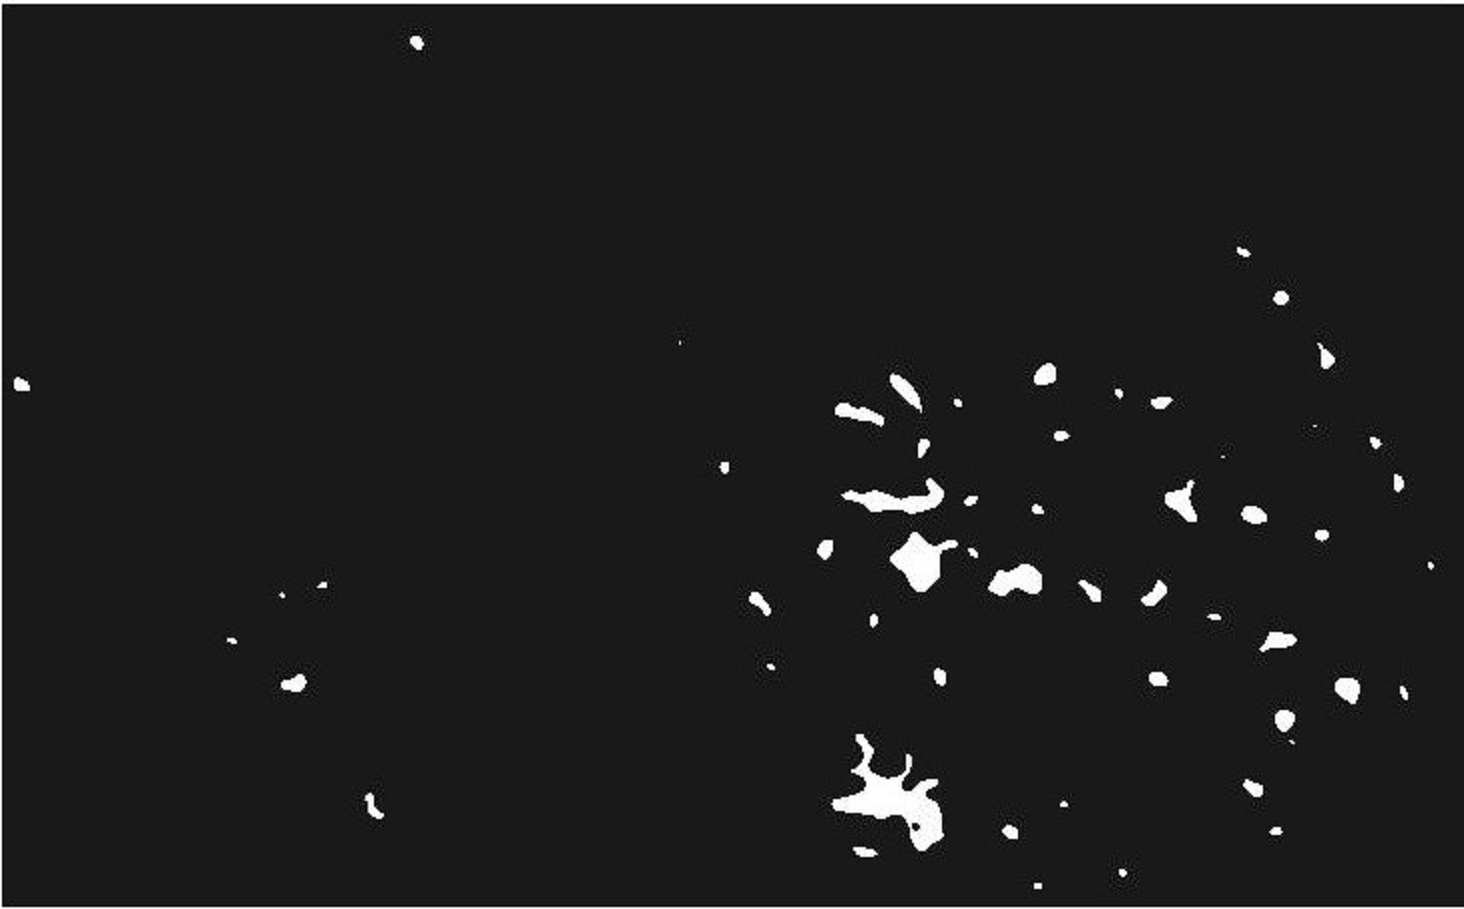
\includegraphics[width=\textwidth]{Imagenes/Homomorfico/ST2_bin.png}
     \hfill
     \caption{Máscara binaria obtenida a partir de la imagen de la figura \ref{sombratorogris} con umbral de 0,45.}
    \label{mascaraST}
\end{figure}

\begin{figure}[h!]
    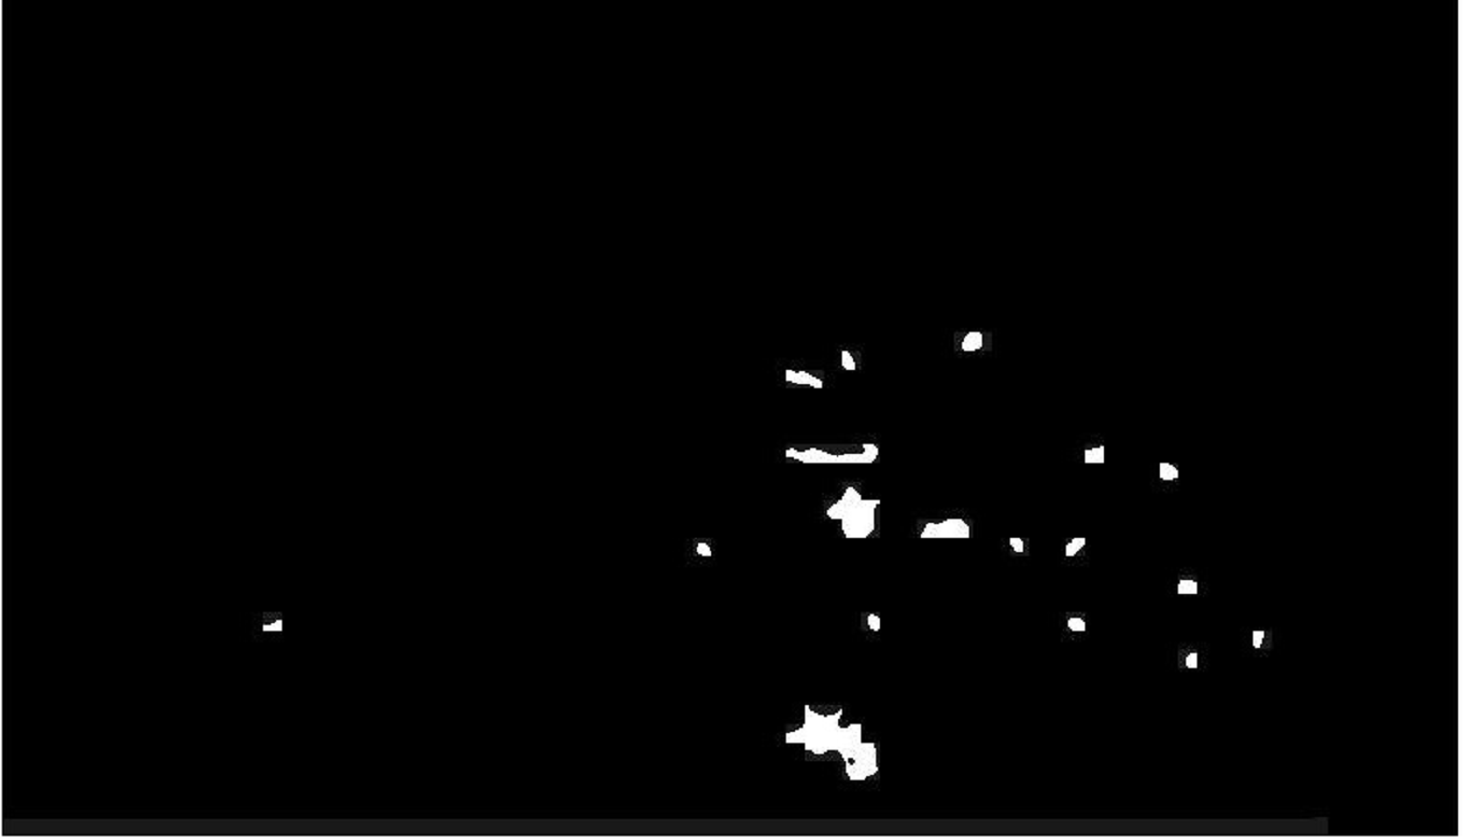
\includegraphics[width=\textwidth]{Imagenes/Homomorfico/ST2_masked.png}
     \hfill
     \caption{Sombras seleccionadas por el algoritmo a partir de la imagen de la figura \ref{mascaraST}.}
    \label{seleccionadaST}
\end{figure}

\begin{figure}[h!]
    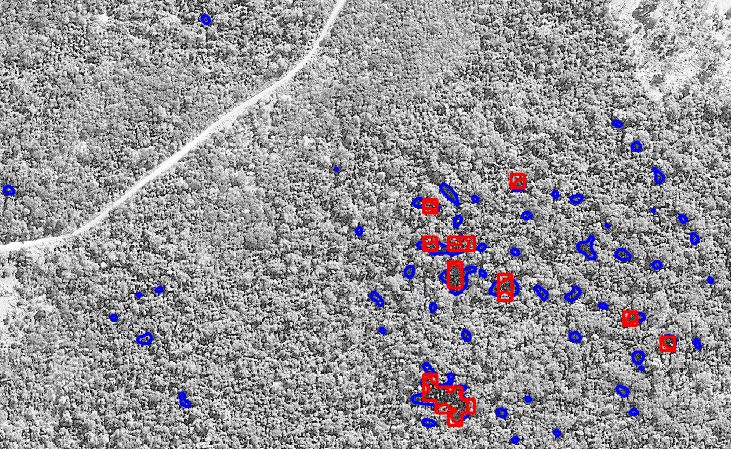
\includegraphics[width=\textwidth]{Imagenes/Homomorfico/ST2_25.png}
     \hfill
     \caption{Superposición de máscara binaria (contorno azul) y máscaras seleccionadas por ventana deslizante (contorno rojo) a la imagen original.}
    \label{ST25}
\end{figure}
%%%%%%%%%%%%%%%%%%%%%%%%%%%%%%%%%%%%%%%%%%%%%%%%%%%%%%%%%%%%%%%%%%%%%%%%%%%%%%%%
\begin{figure}[h!]
    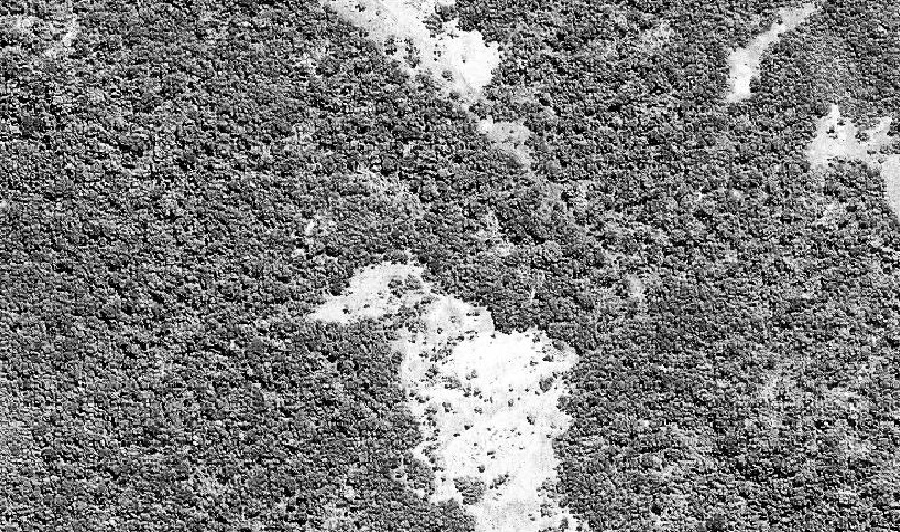
\includegraphics[width=\textwidth]{Imagenes/Homomorfico/PS1_original.jpg}
     \hfill
     \caption{Imagen aérea (satelital) de reserva Parque de la Sierra (identificada como PS1 en la tabla), en escala de grises. Resolución de imagen de 1464 x 900 píxeles, resolución espacial de 0,5 m por pixel.}
    \label{PS1}
\end{figure}

\begin{figure}[h!]
    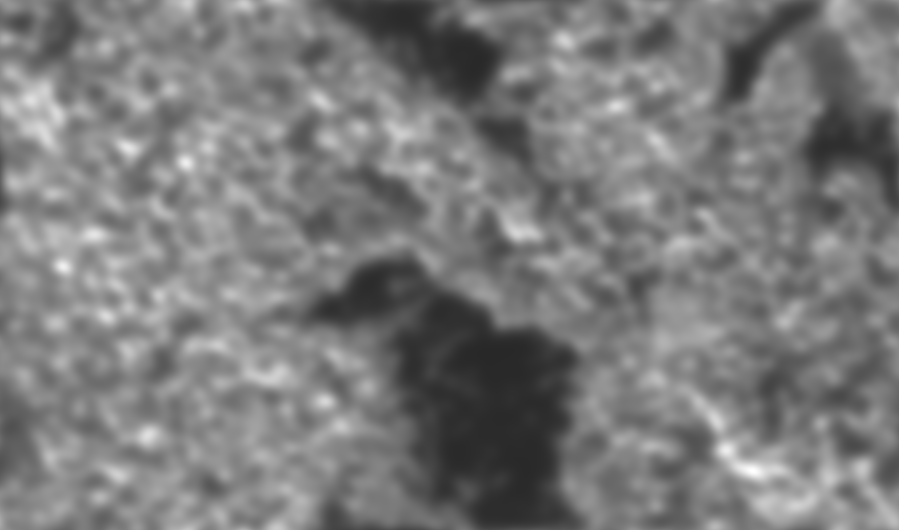
\includegraphics[width=\textwidth]{Imagenes/Homomorfico/PS1_filtered.png}
     \hfill
     \caption{Imagen filtrada con procesamiento homomórfico a partir de la imagen de la figura \ref{PS1}}
    \label{PS1 filtrada}
\end{figure}

\begin{figure}[h!]
    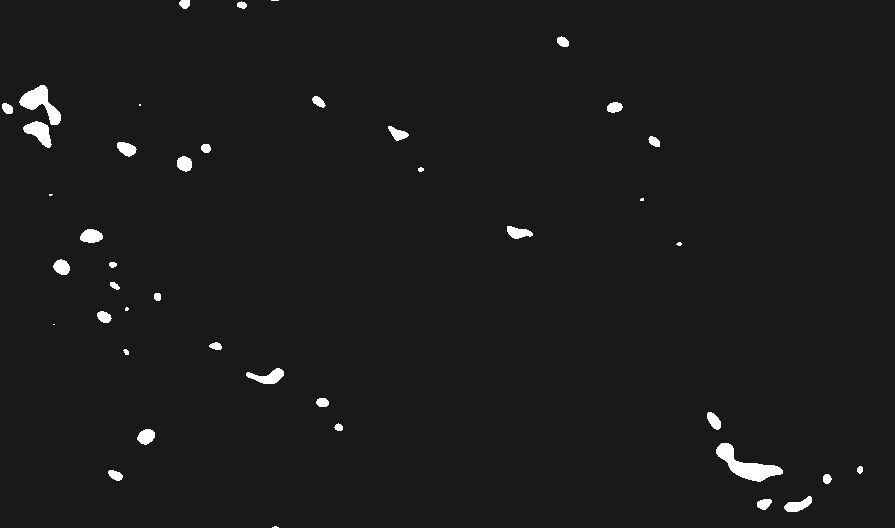
\includegraphics[width=\textwidth]{Imagenes/Homomorfico/PS1_bin.png}
     \hfill
     \caption{Máscara binaria obtenida a partir de la imagen de la figura \ref{PS1 filtrada} con umbral de 0,75.}
    \label{mascaraPS1}
\end{figure}

\begin{figure}[h!]
    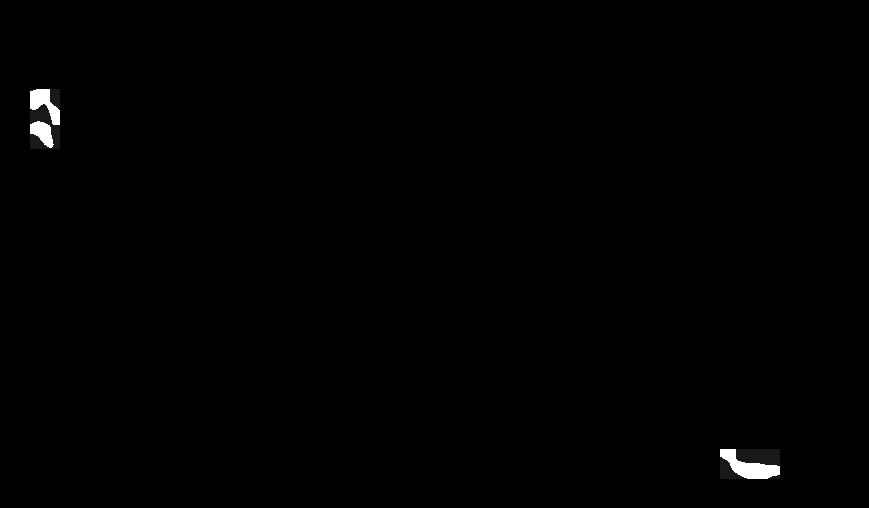
\includegraphics[width=\textwidth]{Imagenes/Homomorfico/PS1_masked.png}
     \hfill
     \caption{Sombras seleccionadas por el algoritmo a partir de la imagen de la figura \ref{mascaraPS1}.}
    \label{seleccionadaPS1}
\end{figure}

\begin{figure}[h!]
    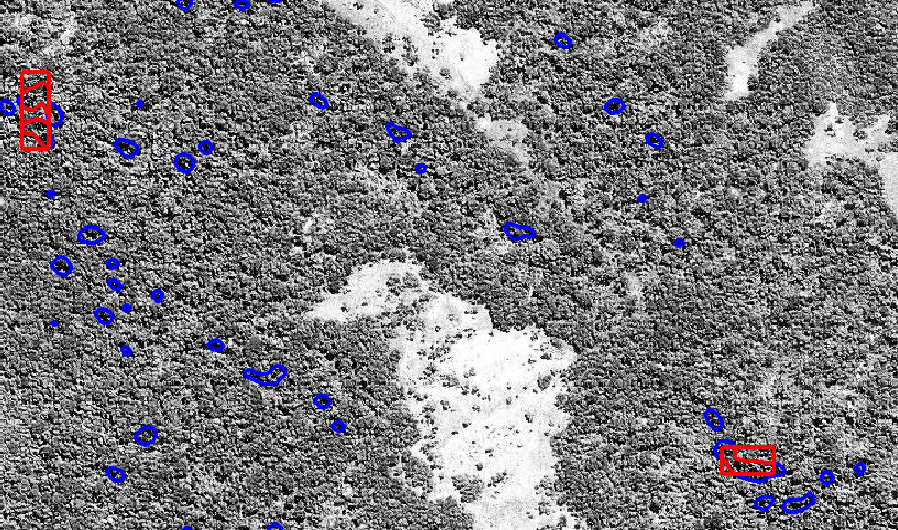
\includegraphics[width=\textwidth]{Imagenes/Homomorfico/PS1_superpuestas.png}
     \hfill
     \caption{Sombras seleccionadas mediante ventana deslizante de tamaño 25 x 25 píxeles a partir de máscara binaria obtenida con umbral de intensidad de 0,75 de la imagen filtrada con procesamiento homomórfico de la figura \ref{PS1}.}
    \label{PS1 superpuesto}
\end{figure}

\subsubsection{Resultados de procesamiento homomórfico y selección automática mediante sistema de inferencia de lógica difusa} \label{resultados homo difusa}
En las figuras \ref{ST2_gris} y \ref{ST2_difuso} se presentan los resultados de la selección automática de sombras obtenida por el algoritmo propuesto en \ref{metod_homo_fuzzy}.
Se muestra la secuencia del procesamiento de la imagen a partir de la imagen original, luego la imagen filtrada, la binarización según el umbral y finalmente la máscara obtenida de acuerdo con los parámetros de selección definidos en el sistema de inferencia difusa.
\begin{figure}[h!]
    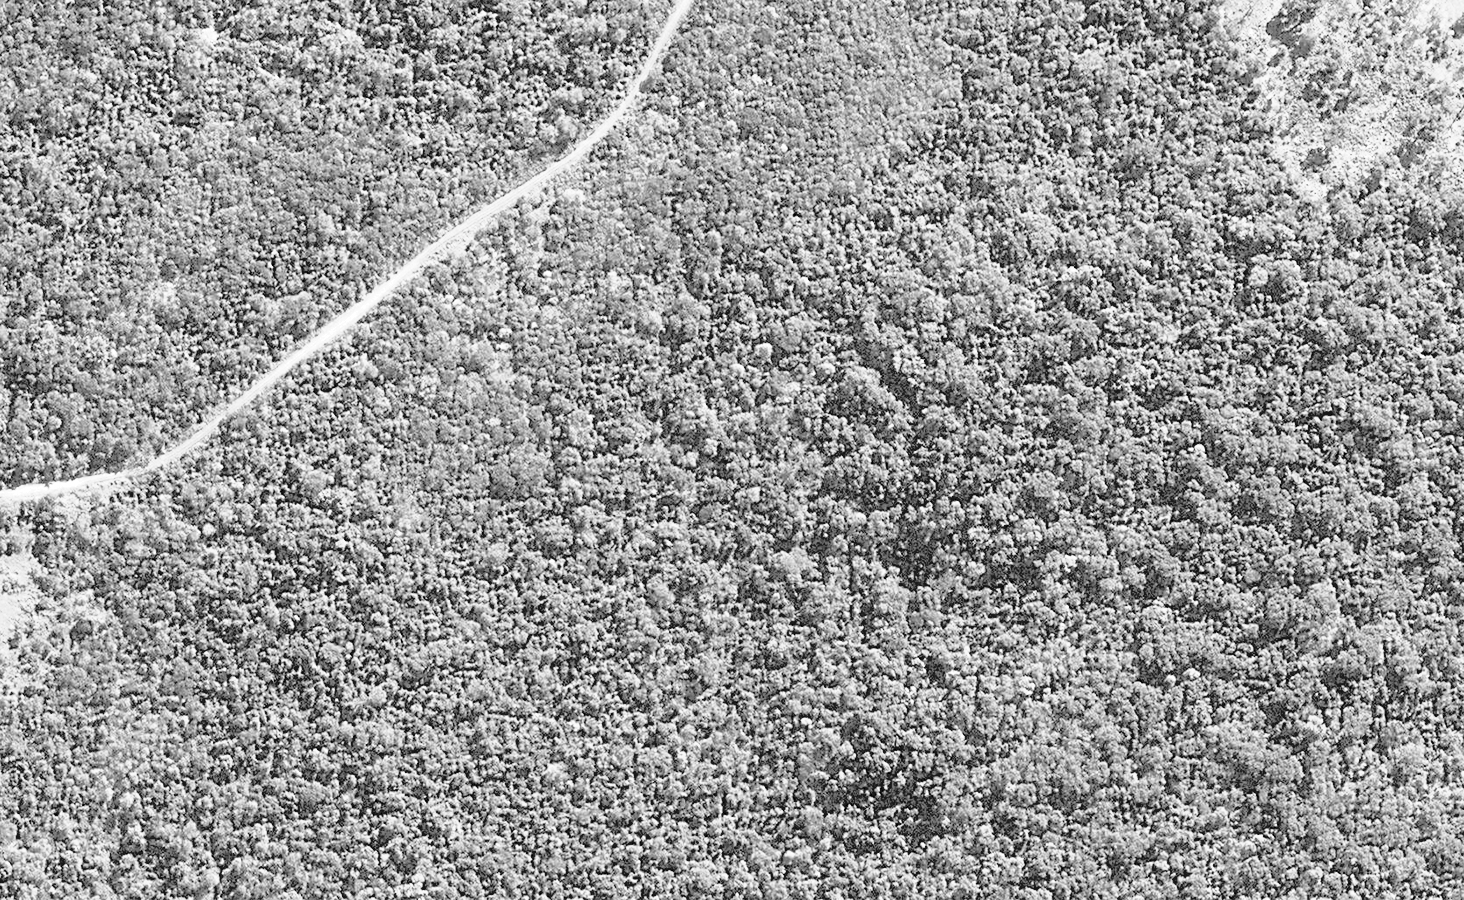
\includegraphics[width=\textwidth]{Imagenes/Homomorfico/ST2.png}
     \hfill
     \caption{Imagen aérea (satelital) de reserva privada Sombra de Toro. Resolución de imagen de 1464 x 900 píxeles, resolución espacial aproximada de  1 m por píxel.}
    \label{ST2_gris}
\end{figure}

\begin{figure}[h!]
    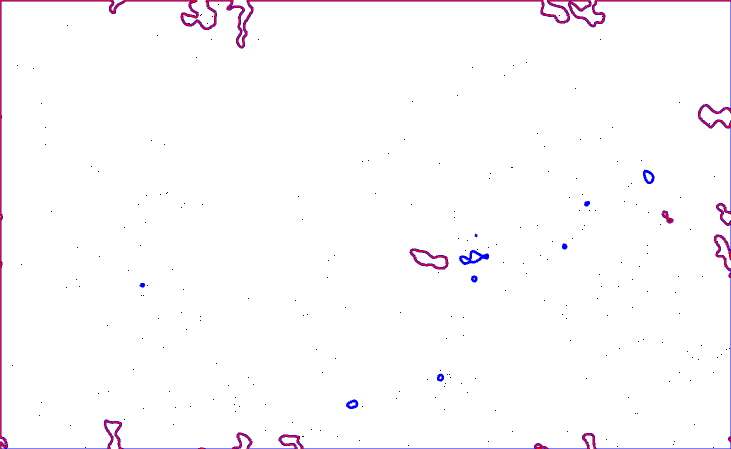
\includegraphics[width=\textwidth]{Imagenes/Homomorfico/ST2_fuzzy.png}
     \hfill
     \caption{Imagen que muestra la selección de sombras realizada por el algoritmo de procesamiento homomórfico con inferencia difusa sobre la figura \ref{ST2_gris}}
    \label{ST2_difuso}
\end{figure}


\begin{figure}[h!]
    \includegraphics[width=\textwidth]{Imagenes/Homomorfico/DJI_0240.JPG}
     \hfill
     \caption{Imagen aérea (VANT) de reserva provincial Cañadón de Profundidad. Resolución de imagen de N x M píxeles, resolución espacial de X m por píxel.}
    \label{Cañadon_homo}
\end{figure}

\begin{figure}[h!]
    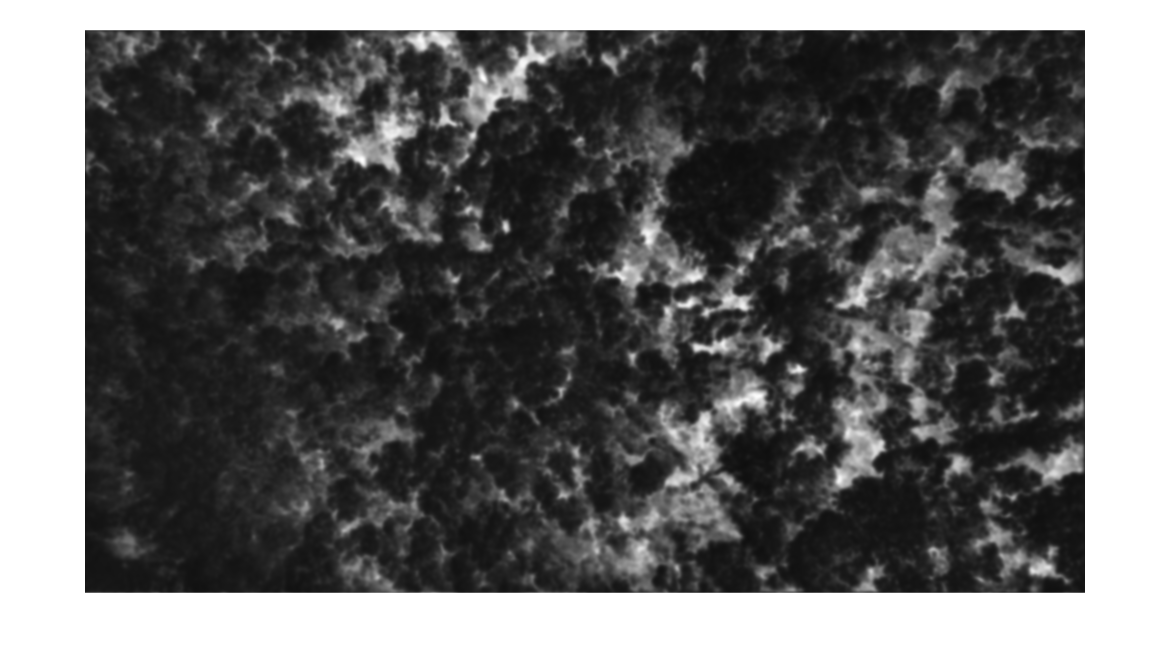
\includegraphics[width=\textwidth]{Imagenes/Homomorfico/dji_240_filter.png}
     \hfill
     \caption{Máscara binaria obtenida a partir de la imagen de la figura \ref{Cañadon_homo} con umbral de 0,45.}
    \label{Cañadon}
\end{figure}

\begin{figure}[h!]
    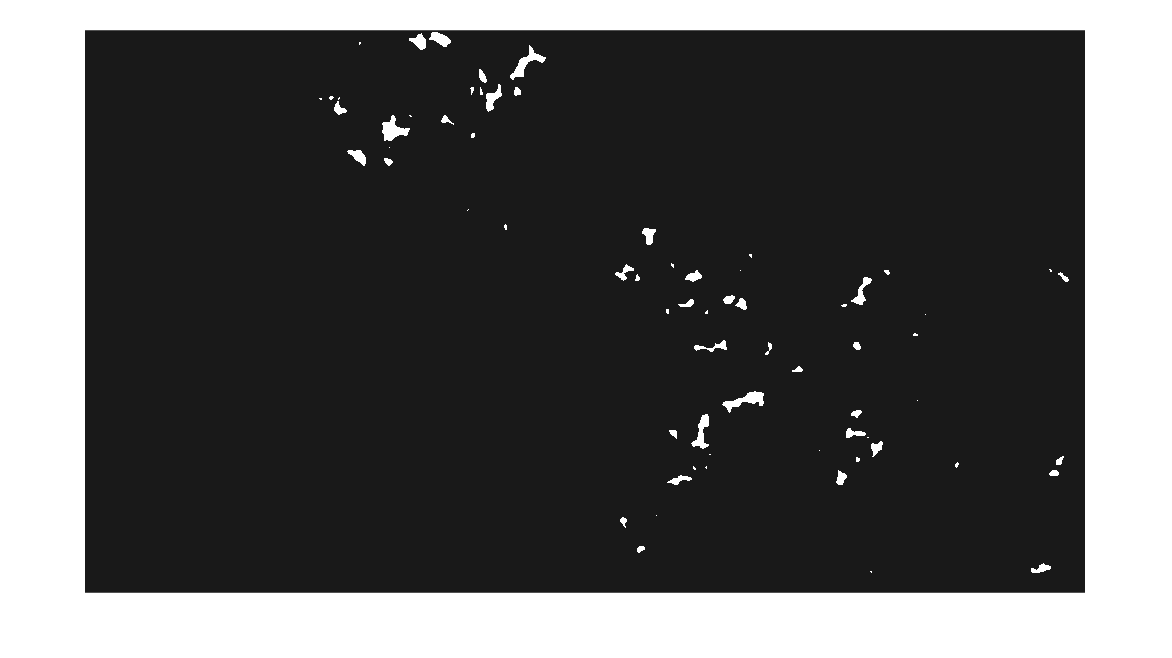
\includegraphics[width=\textwidth]{Imagenes/Homomorfico/DJI_240_bin.png}
     \hfill
     \caption{Máscara binaria obtenida a partir de la imagen de la figura \ref{Cañadon_homo} con umbral de 0,45.}
    \label{mascaraCañadon}
\end{figure}

\begin{figure}[h!]
    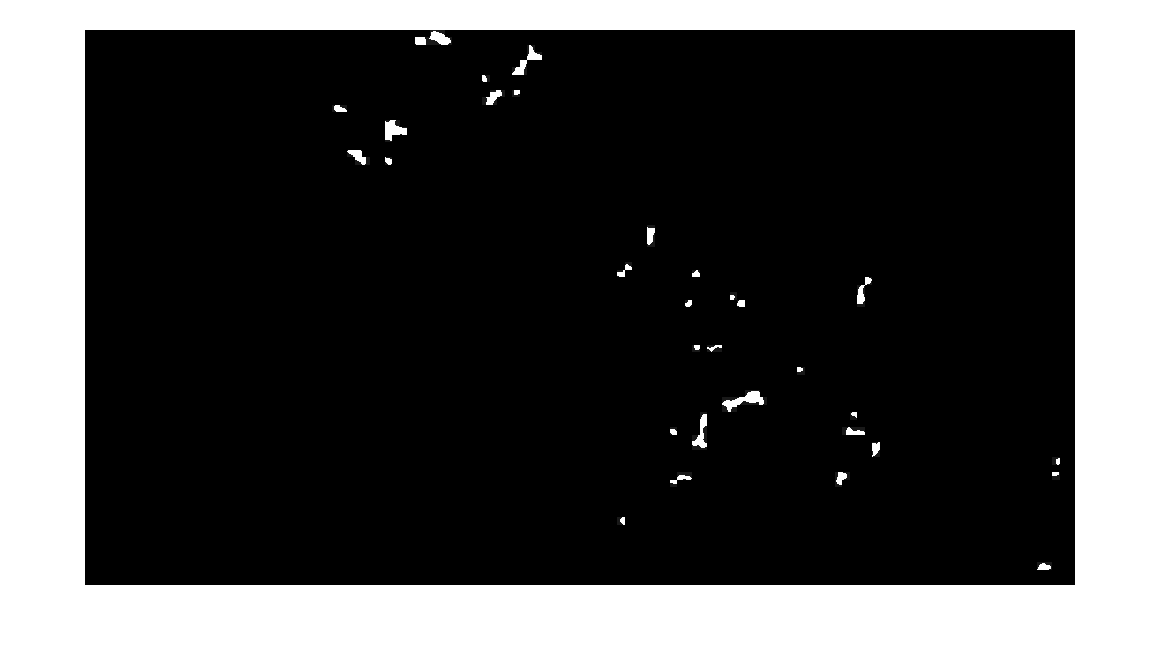
\includegraphics[width=\textwidth]{Imagenes/Homomorfico/DJI_240_sel.png}
     \hfill
     \caption{Sombras seleccionadas por el algoritmo a partir de la imagen de la figura \ref{mascaraCañadon}.}
    \label{seleccionadaDJI240}
\end{figure}

\begin{figure}[h!]
    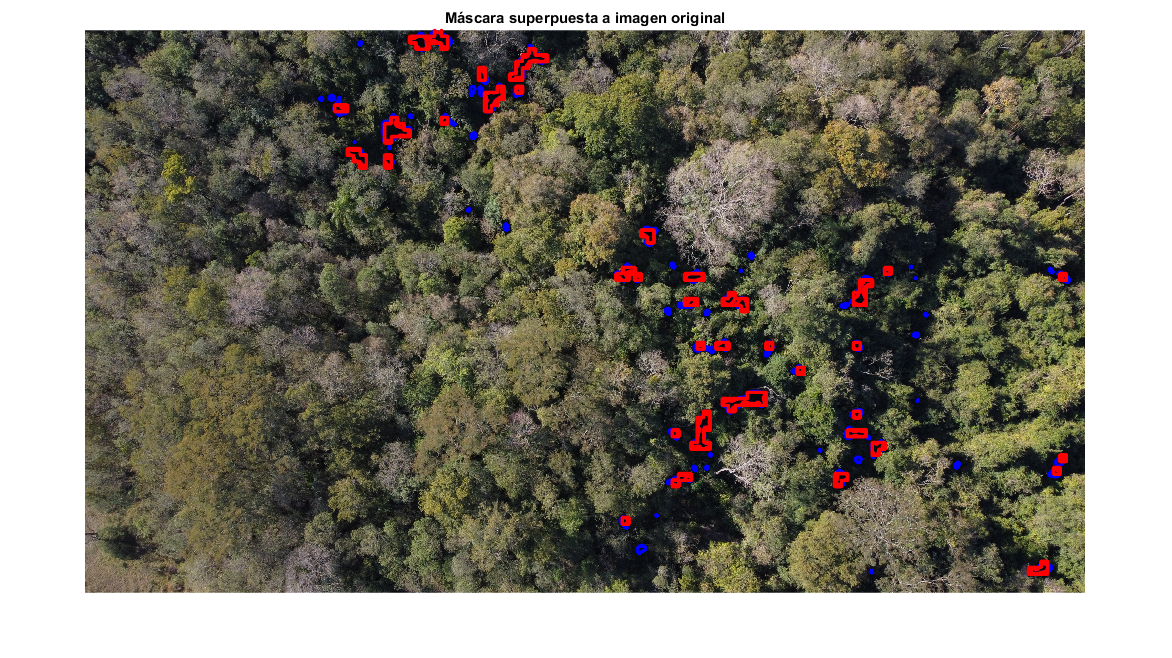
\includegraphics[width=\textwidth]{Imagenes/Homomorfico/dji_240_seleccionadas.png}
     \hfill
     \caption{Máscara binaria obtenida a partir de la imagen de la figura \ref{Cañadon_homo} con umbral de 0,45.}
    \label{mascaraCañadon}
\end{figure}

\begin{figure}[h!]
    \includegraphics[width=\textwidth]{Imagenes/Homomorfico/DJI_0340.JPG}
     \hfill
     \caption{Imagen aérea (VANT) de reserva provincial Cañadón de Profundidad. Resolución de imagen de N x M píxeles, resolución espacial de X m por píxel.}
    \label{Cañadon_homo2}
\end{figure}

\begin{figure}[h!]
    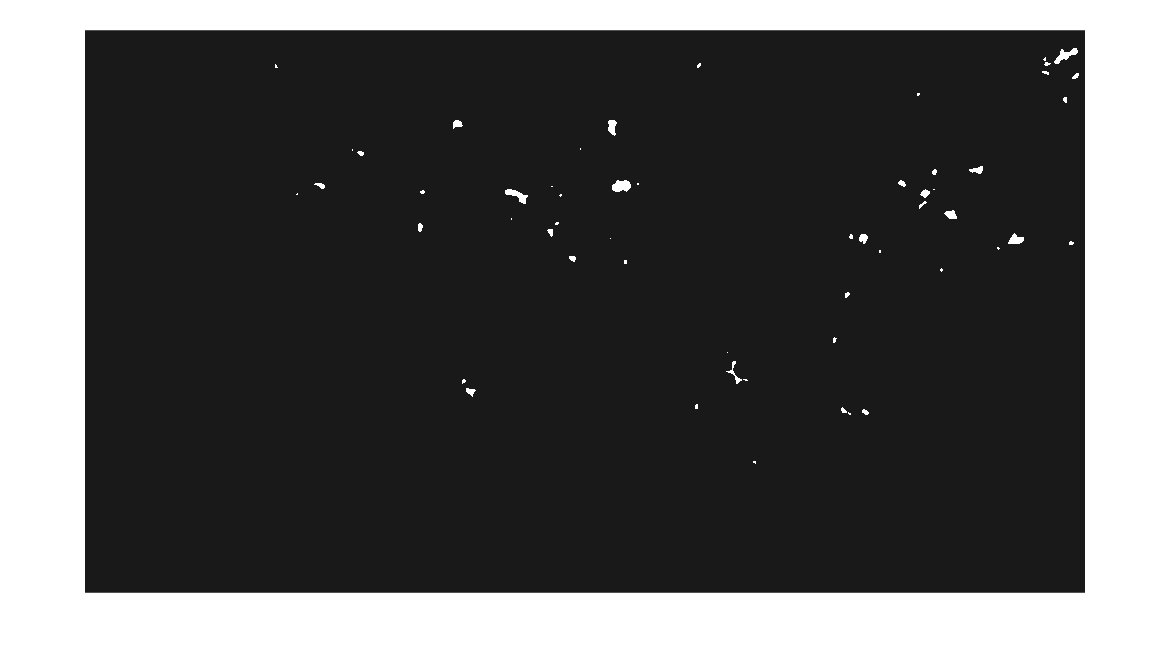
\includegraphics[width=\textwidth]{Imagenes/Homomorfico/DJI_340_bin.png}
     \hfill
     \caption{Máscara binaria obtenida a partir de la imagen de la figura \ref{Cañadon_homo} con umbral de 0,45.}
    \label{mascaraCañadon2}
\end{figure}

\begin{figure}[h!]
    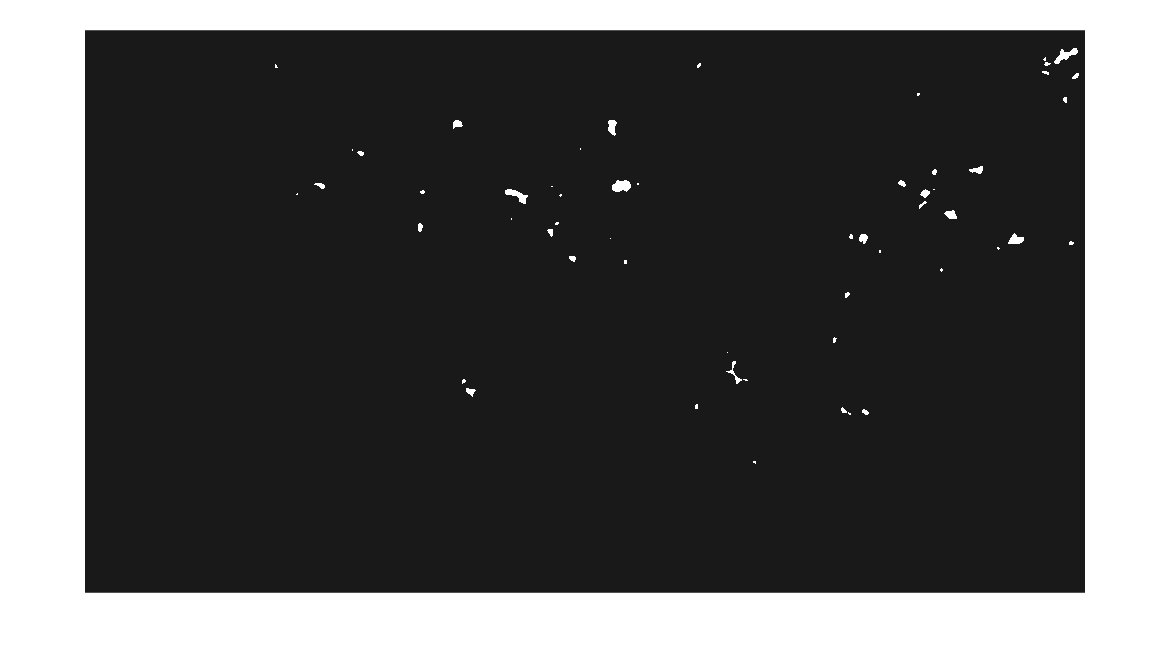
\includegraphics[width=\textwidth]{Imagenes/Homomorfico/DJI_340_bin.png}
     \hfill
     \caption{Sombras seleccionadas por el algoritmo a partir de la imagen de la figura \ref{mascaraCañadon}.}
    \label{seleccionadaCañadon2}
\end{figure}

\subsubsection{Discusión de resultados del procesamiento homomórfico}
%Particular hacia general... cambiar orden, destacar figuras 4.11 a 4.14
%Presentar imagen en el texto. (no dejar imagenes huerfanas)

Según lo observado en los resultados, especialmente en las figuras \ref{Cañadon_homo} y \ref{Cañadon_homo2}, es evidente que el algoritmo requiere de optimización y de concederle mayor robustez ante variaciones en, por ejemplo, la resolución espacial. Los parámetros del algoritmo han sido ajustados para las características de las imágenes satelitales utilizadas. En cuanto se aplicaba el algoritmo con imágenes obtenidas por VANT, los resultados obtenidos diferían de manera considerable, por lo que el algoritmo requería de un ajuste mayor de los parámetros para esas condiciones. De este modo, la automatización de la selección de sombras se ve limitada por las condiciones de las imágenes a ser analizadas.\\
Por otro lado el algoritmo de selección por ventana presenta el inconveniente de que puede tomar un grupo de píxeles discontinuos y considerarlos como una sombra cuando podrían ser dos. Esto obviamente impacta en el resultado del conteo, aparentando menos cantidad de sombras de lo que el ojo humano percibe como tal.                                                                                                                              

%\color{cyan} %color de texto con 70-80 % o más de avance
\subsection{Análisis para conteo de copas de árboles según procesamiento morfológico} \label{resultados morfologico}
En esta subsección se muestran resultados de un análisis de desempeño de un algoritmo de procesamiento morfológico de imágenes de selva según la secuencia presentada en la subsección \ref{Metodo Morfo}, aplicado para establecer la delineación y conteo de copas individuales en el dosel selvático. Se establecieron diferentes valores para un conjunto de parámetros del algoritmo con el objetivo de observar y analizar su influencia en los resultados obtenidos.
Con base en el trabajo realizado por \cite{hubert_wagner_individual_2018}, se llevó a cabo un análisis de desempeño del algoritmo de procesamiento morfológico de imágenes mediante la técnica de búsqueda por grilla, evaluando diferentes valores de parámetros como ser tamaño de ventana, percentil para selección de objetos oscuros y tamaño de objetos para discriminar huecos en copa. En la figura \ref{Rollingball} se muestran los resultados del análisis para diferentes tamaños de ventana en  píxeles, que corresponde a la etapa 4. En la figura \ref{segundaoscuros} se visualizan los resultados para distintos valores de percentil en la etapa de segunda selección de objetos oscuros, correspondiente a la etapa 6. En la figura \ref{pequenoshuecos} se observan los resultados del procesamiento para hallar pequeños huecos en grandes copas, usando distintos valores de percentil, correspondiente a la etapa 7. 

\begin{figure}[h!]
    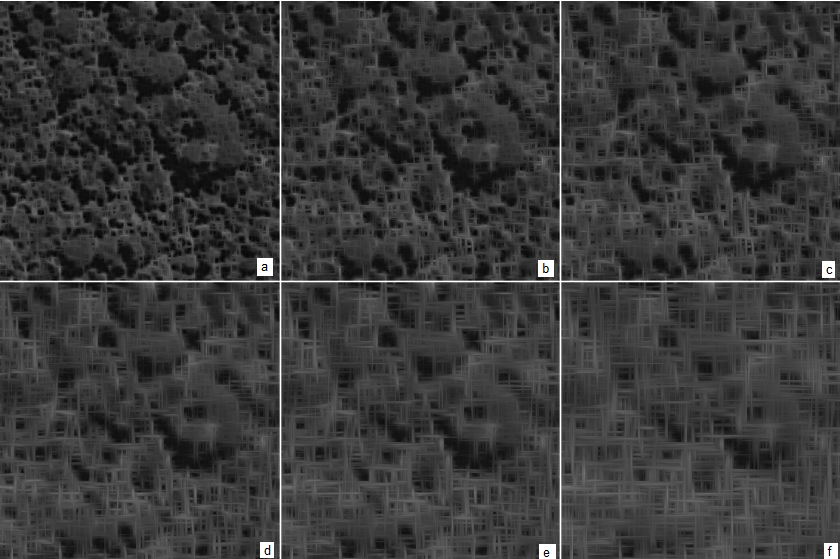
\includegraphics[width=\textwidth]{Imagenes/Resultados script morfologico/GS04-labeled.png}
     %\hfill
     \caption{Resultado del algoritmo Rollingball para tamaños de ventana de a) 6, b) 9, c) 12, d) 15, e) 18 y f) 24 píxeles}
    \label{Rollingball}
\end{figure}
%-------------------------------------------------------------------------------------------------------
\begin{figure}[h!]
    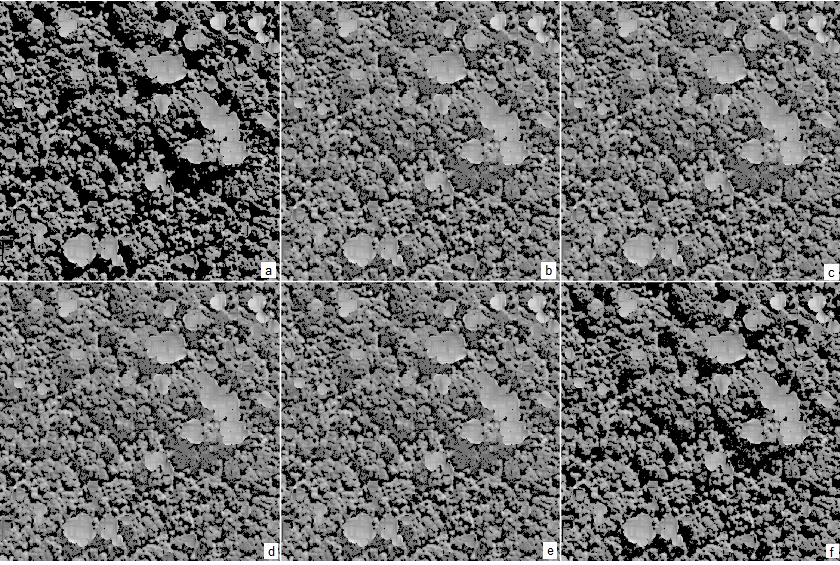
\includegraphics[width=\textwidth]{Imagenes/Resultados script morfologico/GS06-labeled.png}
     %\hfill
     \caption{Resultado de la segunda selección de objetos oscuros con distintos valores de percentil, a) 99, b) 0,1, c) 1, d) 10, e) 50 y f) 90 }
    \label{segundaoscuros}
\end{figure}
%-------------------------------------------------------------------------------------------------------
\begin{figure}[h!]
    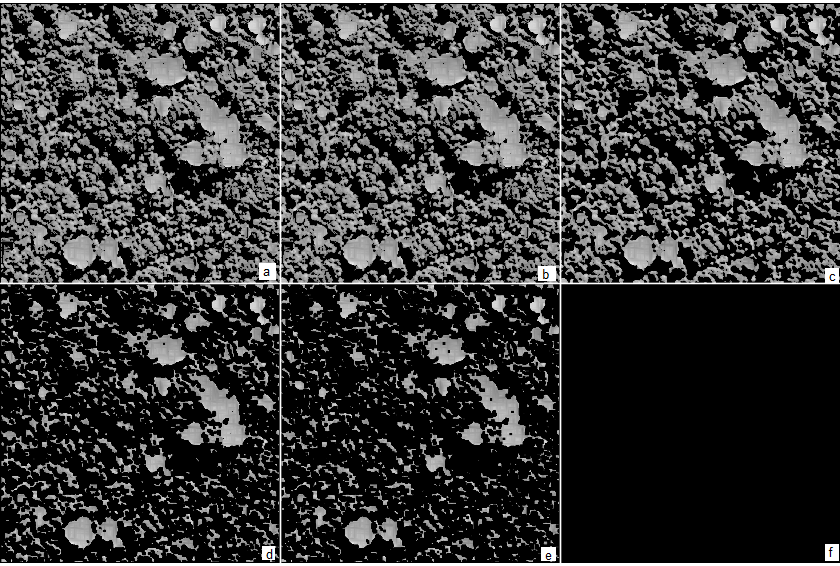
\includegraphics[width=\textwidth]{Imagenes/Resultados script morfologico/GS07-labeled.png}
     %\hfill
     \caption{Resultado de la búsqueda de pequeños huecos con distintos valores de percentil, a) 10, b) 30, c) 50, d) 75, e) 80 y f) 90 }
    \label{pequenoshuecos}
\end{figure}
%-------------------------------------------------------------------------------------------------------
\begin{figure}[h!]
    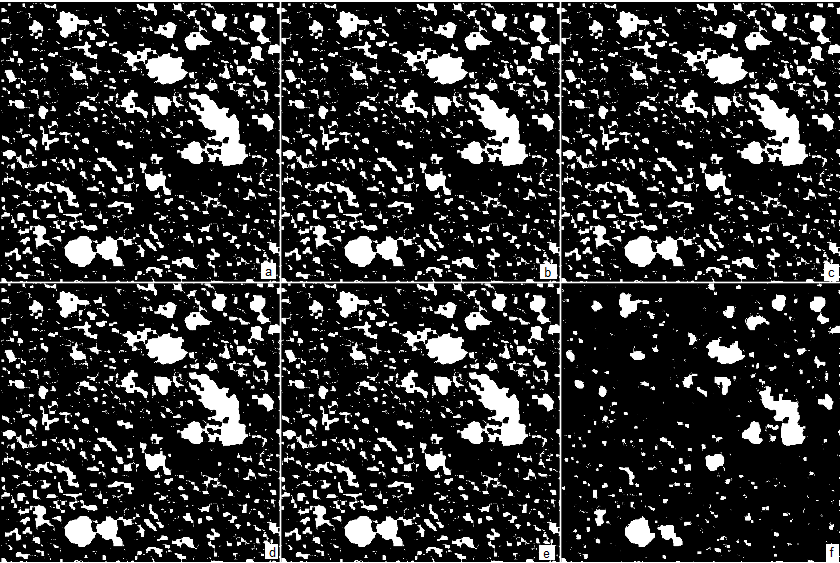
\includegraphics[width=\textwidth]{Imagenes/Resultados script morfologico/GS09-labeled.png}
     %\hfill
     \caption{Resultado del filtrado con topbottom y binarizado con distintos valores de percentil, a) 0,1, b) 1, c) 10, d) 20, e) 50 y f) 90 }
    \label{topbottom}
\end{figure}

\subsubsection{Evaluación de la influencia de diferentes parámetros en los algoritmos}
Se evaluó el desempeño de los algoritmos modificando en un determinado rango el valor de distintos parámetros en cada etapa del procesamiento, para observar en qué modo se ven afectados los resultados y la vinculación que tienen los parámetros en las diferentes etapas con la resolución espacial de la imagen con la que se trabaja. En tanto, en la última etapa se observó que el umbral
que se definió para separar (y por lo tanto binarizar la imagen) las copas segmentadas, en el artículo de referencia sugiere utilizar el umbral del 0,1º percentil, pero al hacer la prueba de \textit{Gridsearch} con diferentes valores hasta el 90º percentil, resultaba notable que excepto el correspondiente al percentil 90º los demás resultados no eran visiblemente
diferentes.

\subsubsection{Discusión}
Para el procesamiento morfológico de imágenes se ha utilizado la herramienta R, mostrado características que merecen ser tenidas en cuenta en el análisis. Por lo general esta herramienta es poderosa para el análisis estadístico de datos, y especialmente útil en datos georreferenciados, pero también muy demandante en términos de recursos computacionales, ya que al procesar los datos en archivos raster, la exigencia de memoria RAM es elevada. Asimismo hay rutinas del proceso analizado que demandan una considerable cantidad de tiempo, incluso varios minutos, como es el caso del comando  normalmixEM() del paquete mixtools (ver \cite{young__aut_mixtools_2022}).


%\color{cyan} %color de texto con 70-80 % o más de avance
\subsection{Resultados del procesamiento por el método de índice invariante de color (IIC)} \label{Resultados IIC}
Un total de diecinueve imágenes aéreas de selva fueron consideradas para realizar el análisis. Dos de ellas representativas de los diferentes escenarios que fueron cubiertos, se muestran en las figuras \ref{calle} y \ref{tupido}. La figura \ref{calle} muestra una imagen en la que unas pocas copas de árboles se distribuyen por el área capturada, mientras que en la \ref{tupido} el dosel cubre prácticamente toda el área. La delineación manual de las sombras fue realizada como se describe en el apartado de \ref{Metodología IIC}
Dos ejemplos de máscaras manuales se muestran en figuras \ref{contorno1} y \ref{contorno2}, con trazo rojo bordeando las regiones sombreadas. Las figuras \ref{p60} y \ref{p85} muestran el solapamiento de la máscara manual (en rojo) con la automática (en azul). En la figura \ref{p60} el valor de umbral para la máscara binaria se toma del 60º percentil de la distribución de frecuencias, mientras que en la figura \ref{p85} el valor de umbral es tomado del 85º percentil.

\begin{figure}[H]
    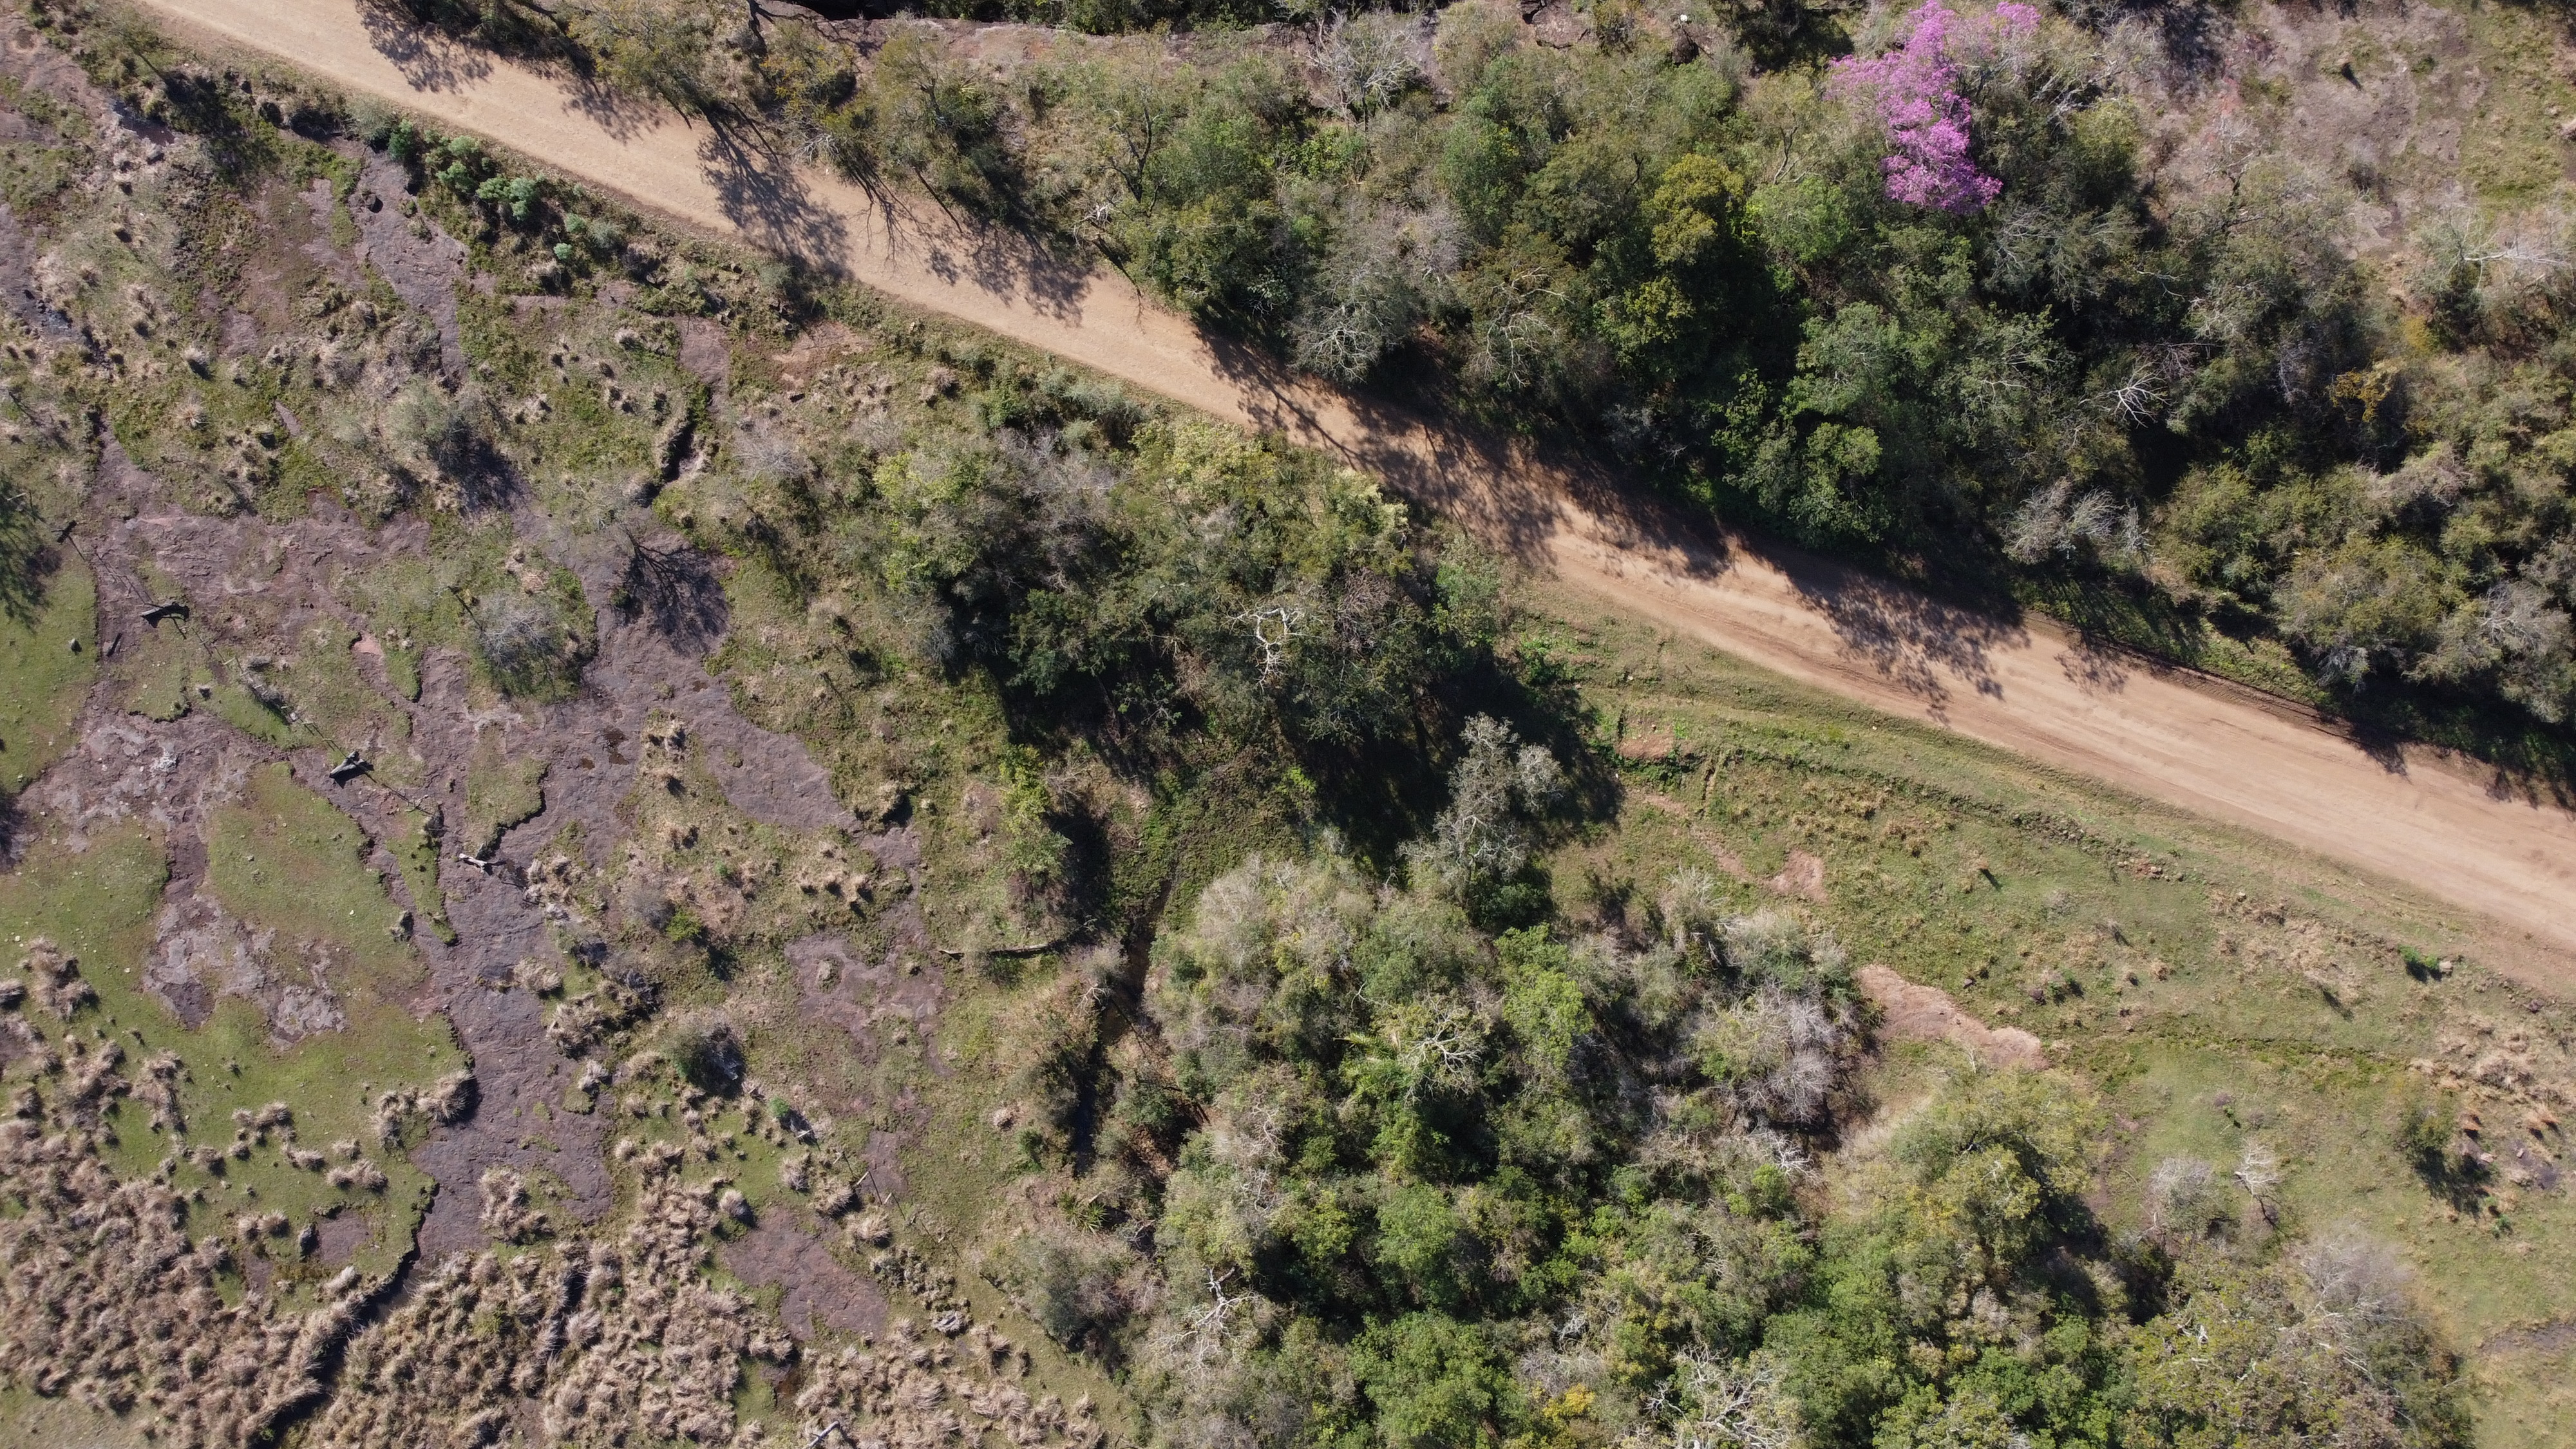
\includegraphics[width=\textwidth]{Imagenes/street.jpg}
     \hfill
     \caption{Escena capturada con pocos árboles}
    \label{calle}
\end{figure}

\begin{figure}[H]
    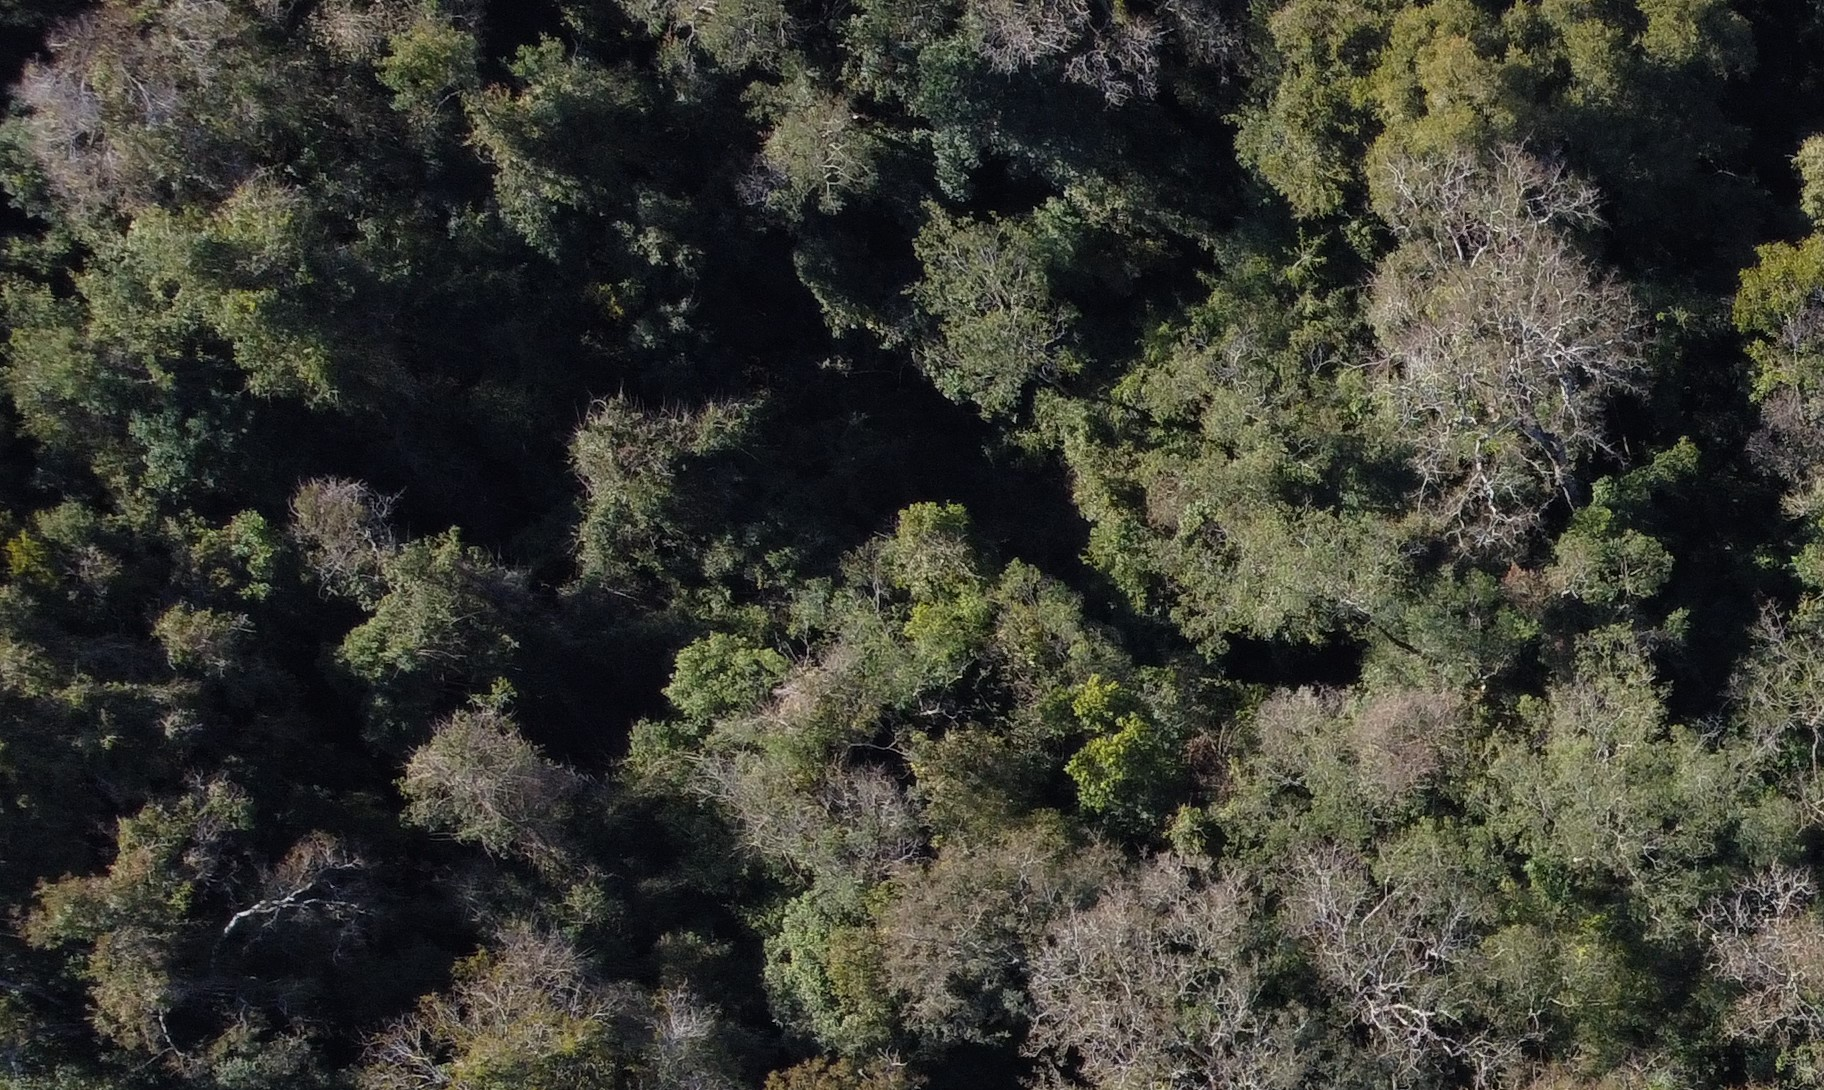
\includegraphics[width=\textwidth]{Imagenes/dense canopy.jpg}
     \hfill
     \caption{Escena capturada con dosel tupido}
    \label{tupido}
\end{figure}


\begin{figure}[H]
    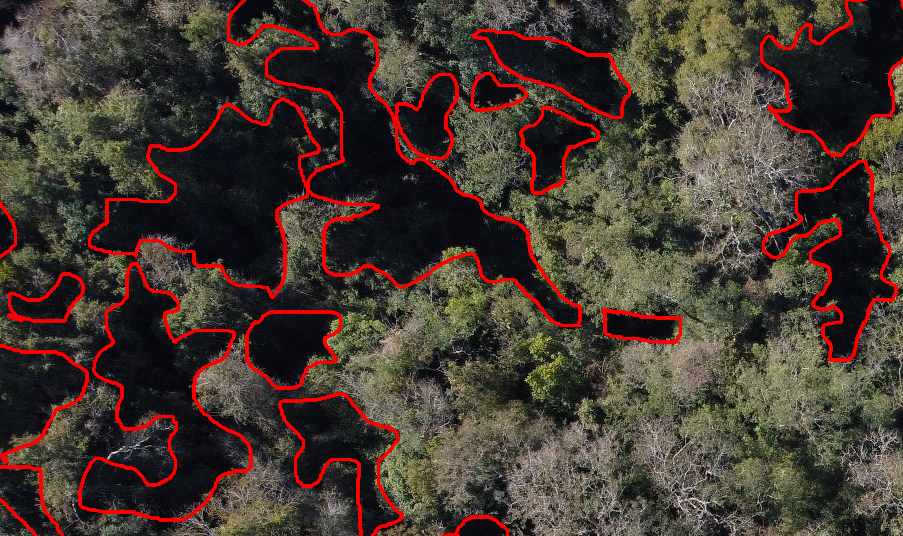
\includegraphics[width=\textwidth]{Imagenes/contours.png}
     \hfill
     \caption{Contornos de sombras en dosel tupido}
    \label{contorno1}
\end{figure}

\begin{figure}[H]
    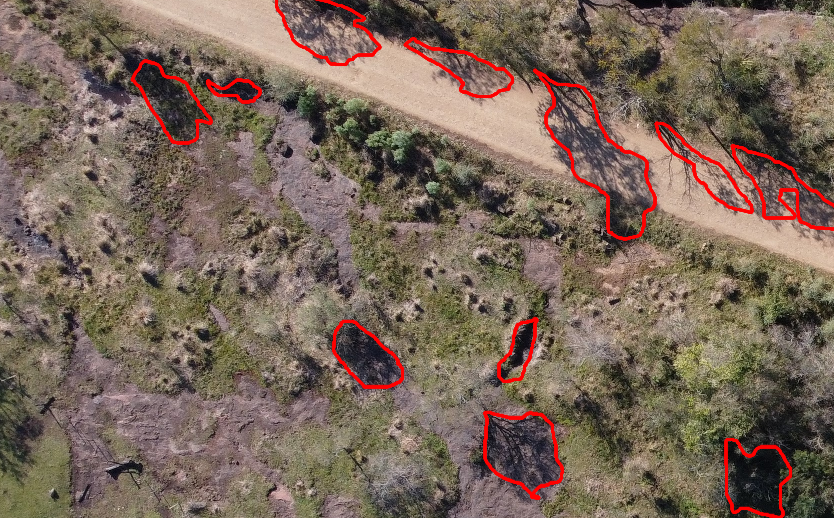
\includegraphics[width=\textwidth]{Imagenes/contours2.png}
     \hfill
     \caption{Contorno de sombras en imagen con pocos árboles}
    \label{contorno2}
\end{figure}

\begin{figure}[H]
     
         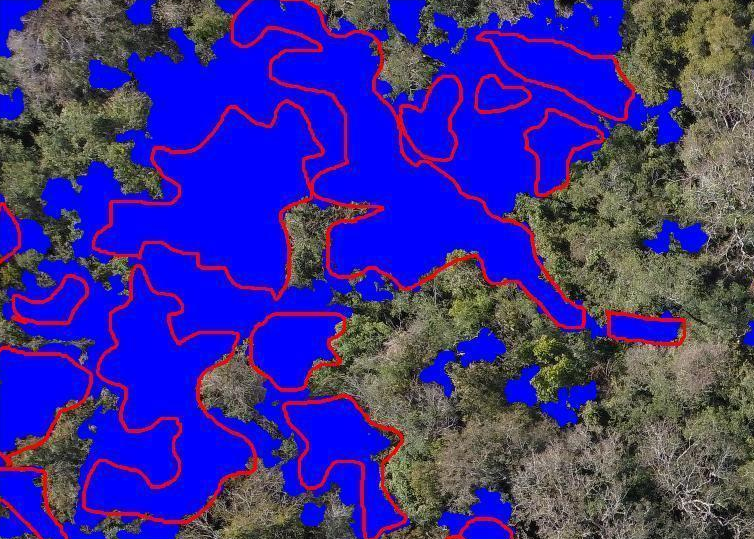
\includegraphics[width=\textwidth]{Imagenes/superposition of masks.png}
         \caption{Superposición de máscaras automática (color azul) y manual (contorno rojo), percentil 60º}
         \label{p60}
\end{figure}
     \hfill
     
\begin{figure}[H]
         
         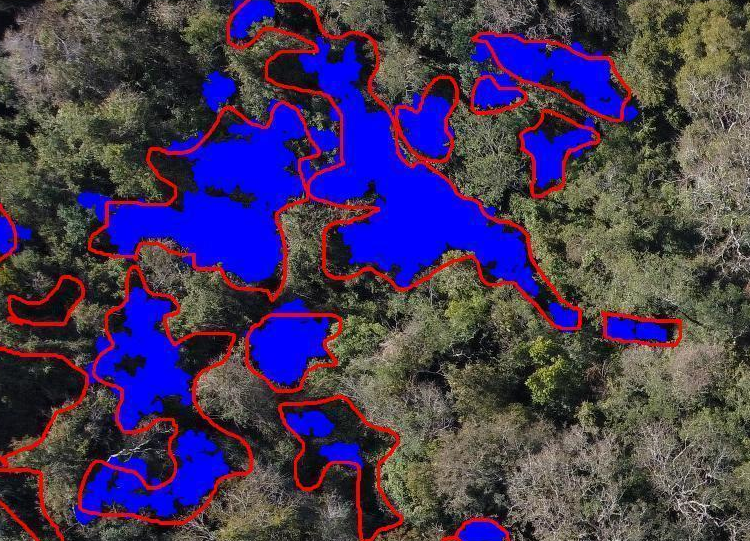
\includegraphics[width=\textwidth]{Imagenes/superposition of masks 2.png}
         \caption{Superposición de máscaras automática (color azul) y manual (contorno rojo), percentil 85º}
         \label{p85}
\end{figure}

\begin{figure}[H]
    
    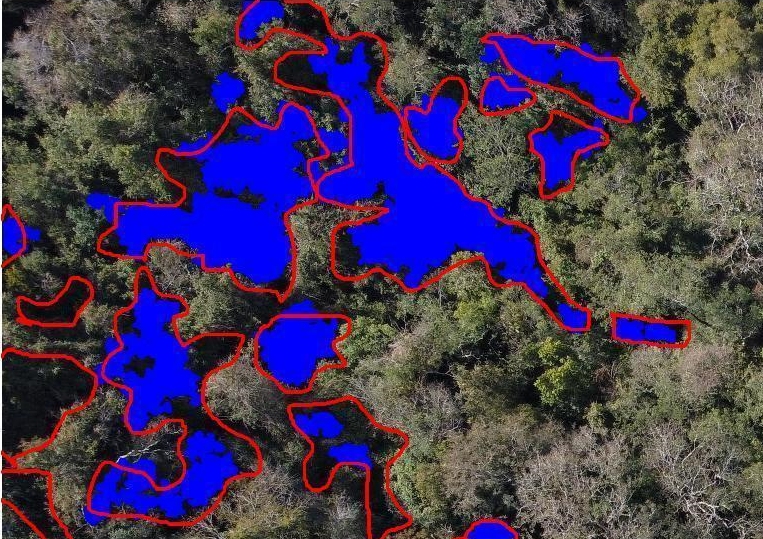
\includegraphics[width=\textwidth]{Imagenes/blue minus red 85.png}
     \hfill
     \caption{Superposición de máscaras automática (color azul) y manual (contorno rojo), percentil 85\textpsi\textsubscript{BR}}
    \label{azulrojo}
 \end{figure}

 \begin{figure}[H]
    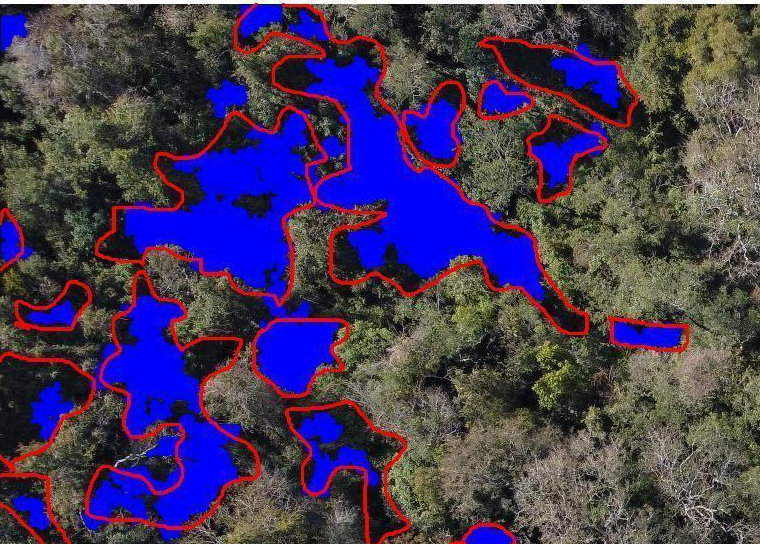
\includegraphics[width=\textwidth]{Imagenes/blue minus green 85.png}
     \hfill
     \caption{Superposición de máscaras automática y manual \textpsi\textsubscript{BG}}
    \label{azulverde}
 \end{figure}

 \begin{figure}[H]
    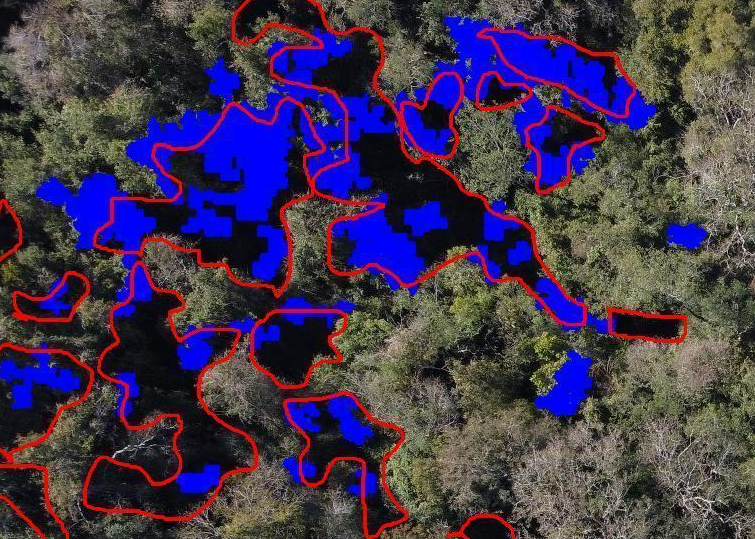
\includegraphics[width=\textwidth]{Imagenes/green minus red 85.png}
     \hfill
     \caption{Superposición de máscaras automática y manual \textpsi\textsubscript{GR}}
    \label{verderojo}
 
\end{figure}

\begin{figure}[H]
    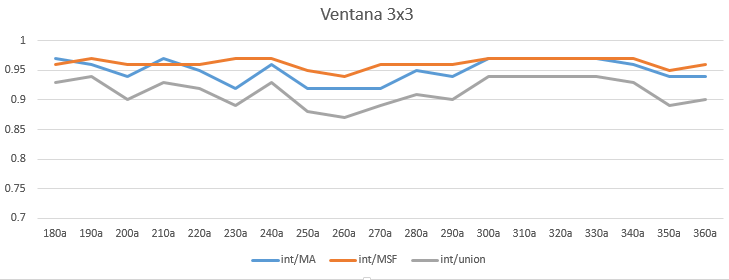
\includegraphics[width=\textwidth]{Imagenes/filter 3x3.png}
     \hfill
     \caption{Filtro 3x3}
    \label{filter3x3}
\end{figure}

\begin{figure}[H]
    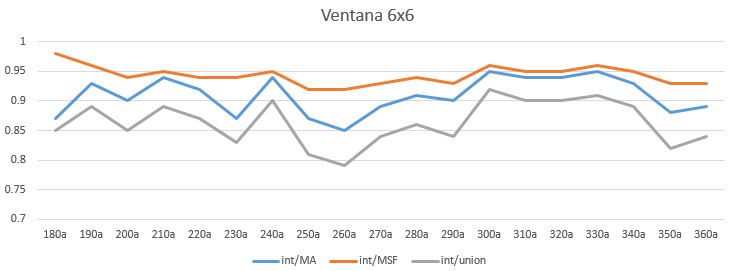
\includegraphics[width=\textwidth]{Imagenes/filter 6x6.png}
     \hfill
     \caption{6x6}
    \label{filter6x6}
\end{figure}

\begin{figure}[H]
    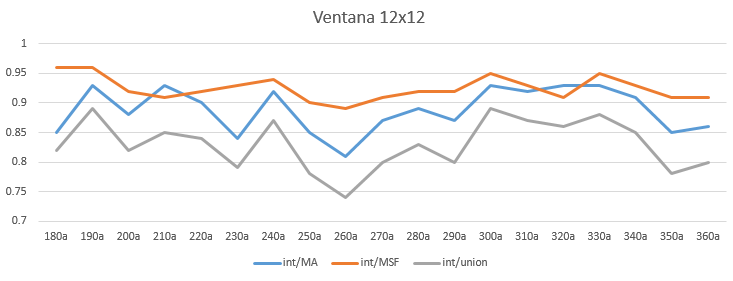
\includegraphics[width=\textwidth]{Imagenes/filter 12x12.png}
     \hfill
     \caption{12x12}
    \label{filter12x12}
\end{figure}
%%%%%%%%%%%%%%%%%%%%%%%%%%%%%%%%%%%%%%%%%%%%%%%%%%%%%%%%%%%%%%%%%%%%%%%%%


%%%%%%%%%%%%%%%%%%%%%%%%%%%%%%%%%%%%%%%%%%%%%%%%%%%%%%%%%%%%%%%%%%%%5

\begin{figure}[H]
    \centering
  \begin{subfigure}[b]{\textwidth}
    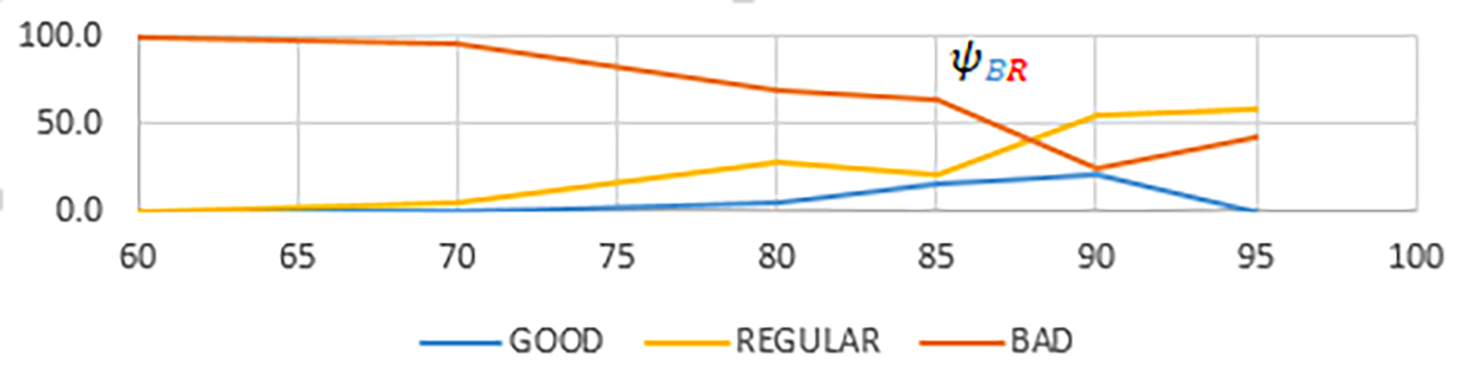
\includegraphics[width=\textwidth]{Imagenes/psiBR.png}
     \hfill
     \caption{Índice $\Psi_{BR}$}
    \label{psiazulrojo}
 \end{subfigure}

 \begin{subfigure}[b]{\textwidth}
    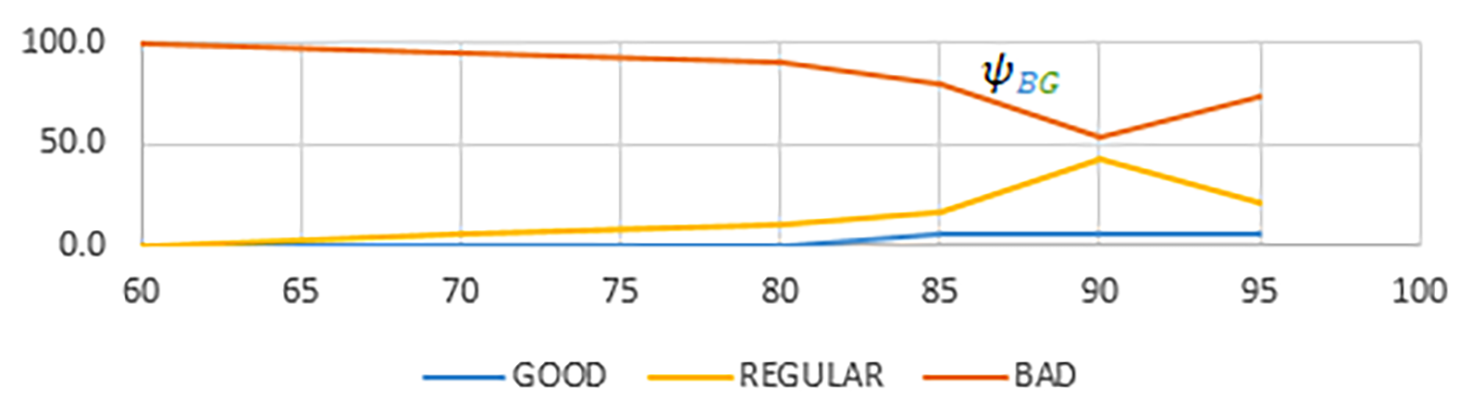
\includegraphics[width=\textwidth]{Imagenes/psiBG.png}
     \hfill
     \caption{Índice $\Psi_{BG}$}
    \label{psiazulverde}
 \end{subfigure}

 \begin{subfigure}[b]{\textwidth}
    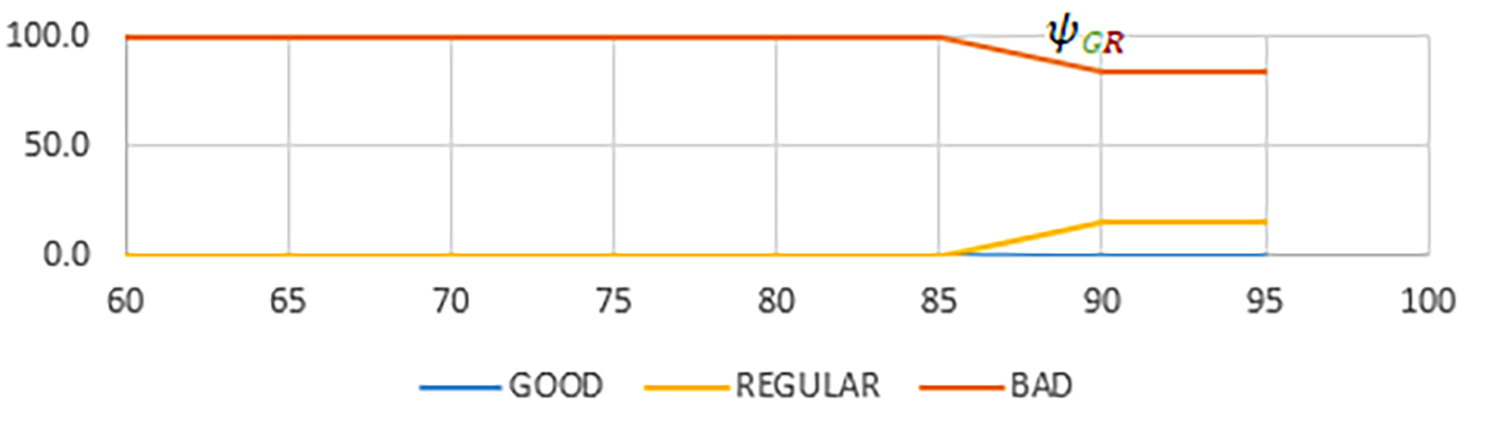
\includegraphics[width=\textwidth]{Imagenes/psiGR.png}
     \hfill
     \caption{Índice $\Psi_{GR}$}
    \label{psiverderojo}
 \end{subfigure}
 \caption{Comparación de máscaras automáticas con manual, para tres casos de índice invariante de color}
        \label{compara_mascara}
\end{figure}

\subsubsection{Influencia del valor de percentil y del índice invariante de color}

La figura \ref{azulrojo}, \ref{azulverde} y \ref{verderojo} muestra para la misma escena, diferentes máscaras automáticas obtenidas con diferentes configuraciones de la ecuación \ref{invariante de color}, usando tres diferentes combinaciones de canales de dos colores. La figura \ref{azulrojo} corresponde a la máscara obtenida usando la diferencia entre el canal azul menos el canal rojo $\Psi_{BR}$, la figura \ref{azulverde} usando la diferencia entre el canal azul menos el canal verde $\Psi_{BG}$ y la figura \ref{verderojo} usando la diferencia entre el canal verde menos el canal rojo $\Psi_{GR}$. En todos los casos el valor de umbral fue tomado del 85º percentil de la distribución de frecuencia. El análisis de las figuras \ref{azulrojo} a \ref{verderojo} muestra que, aplicando la ecuación \ref{invariante de color} usando ya sea la combinación de canales azul con verde $\Psi_{BG}$ o azul con rojo $\Psi_{BR}$  las máscaras automáticas resultantes para un mismo valor de percentil son de área mayor que las que corresponden al índice calculado con la diferencia entre canal verde y rojo $\Psi_{GR}$, lo que resulta en valores de QI más altos para $\Psi_{BR}$ y $\Psi_{BG}$ que para $\Psi_{GR}$. La comparación entre las distintas influencias del valor de percentil puede observarse en la figura \ref{curvas_QI}, donde resulta evidente que $QI_1$ es el más alto en el percentil bajo 60º y $QI_2$ es el más alto para el percentil alto 95º. 

Por otro lado el índice $QI_3$ se asemeja a una curva convexa, con valores similares a $QI_1$ para el percentil 60º y similares a $QI_2$ para el percentil 95º, cuyo valor máximo en la curva corresponde al 85º percentil. Un comportamiento similar se observa para los otros índices invariantes de color $\Psi_{BG}$ y $\Psi_{GR}$. La similitud entre QI1 y QI2 en el percentil más bajo se debe al hecho de que la máscara automática selecciona un área de sombra que resulta preponderante en la operación de unión binaria en el denominador de la ecuación \ref{qi3} en el caso de $QI_3$.
Por otro lado, el índice $QI_3$ se aproxima a $QI_1$ cuando la máscara automática selecciona un área pequeña de sombra, por lo tanto la selección manual de sombra resulta dominante en la operación de unión de máscaras en el denominador de la ecuación \ref{qi3}.
Al maximizar la intersección, se asegura la coincidencia entre las máscaras manual y automática, pero podría excederse en la máscara automática. Luego, al minimizar la unión, se puede controlar el tamaño pleno de la máscara automática. Un punto óptimo es el caso en el que el índice $QI_3$ alcanza el máximo valor. A pesar de la dispersión de los datos (ver figura \ref{curvas_QI}), se puede analizar los valores medios de los índices de calidad QI para los tres casos considerados (ver figuras \ref{psiBR}, \ref{psiBG}, \ref{psiGR}). Se observa que el valor que corresponde al 85º percentil de la distribución de frecuencia del índice invariante de color es el óptimo, ya que corresponde a un máximo del índice $QI_3$.

En el análisis de la figura \ref{quality_index}, se observan grandes similitudes, donde se grafican las relaciones entre los tres índices de calidad propuestos y un índice adicional definido como la diferencia entre el valor máximo y el mínimo entre los tres índices en función del valor de percentil usado para calcular el umbral de la máscara binaria automática. En los tres casos se detecta un valor mínimo para la curva que corresponde al índice adicional, es decir el rango (max - min), y este valor mínimo corresponde al percentil 85º. Además para los casos que usan sendas combinaciones en la ecuación \ref{invariante de color} resta de canal azul menos rojo y azul menos verde, la curva del índice $QI_3$ alcanza un valor máximo en el que corresponde al 85º percentil, mientras que este punto máximo no se hace evidente para el caso de de la combinación verde menos rojo. Por lo tanto de los cuatro índices que fueron analizados, el más conveniente es el $QI_3$, que exhibe un valor óptimo de percentil más preciso por medio del mínimo en la curva, y en los tres casos de combinaciones de canales es coincidente.

\subsubsection{Influencia del filtro de mediana en la detección automática de sombras}

La figura \ref{filter3x3}, \ref{filter6x6} y \ref{filter12x12} muestra cómo los índices que son obtenidos por las ecuaciones \ref{qi5} a \ref{qi7} son afectados por la implementación del filtro de mediana a cada imagen. En el caso del filtro de 3 x 3 píxeles, que tiene menor incidencia en los índices, los índices de calidad tienen valores mayores al 85\% para todas las imágenes. El peor desempeño lo tiene el filtro de 12 x 12, cuyo resultado comparado con la máscara automática obtenida sin filtro arrojaba una coincidencia de poco más que el 70\%.

\subsubsection{Evaluación humana de máscaras automáticas de sombra}

En este trabajo los resultados del algoritmo se comparan con la selección manual llevada a cabo por expertos. Partiendo de que no hay una base de certeza absoluta (los expertos son personas humanas y por lo tanto proclives a errores de omisión o comisión), existe una limitación en el índice de calidad que se basa en este aspecto. El criterio para la selección manual de parte de los expertos depende de su particular percepción de la imagen, variando según el contexto. Por otro lado el algoritmo se basa en el cálculo de un índice y la definición de un valor umbral, obtenido de una serie de experimentos con imágenes de un determinado tipo. En otros contextos con otro tipo de imágenes el valor de umbral no sería el mismo, incluso la combinación de bandas usadas en la ecuación \ref{invariante de color} para obtener el índice sería diferente.

Luego de generar un conjunto de máscaras correspondientes a cada uno de los seis percentiles usando los tres índices invariantes de color de las ecuaciones \ref{psibr} a \ref{psigr} para las 19 imágenes seleccionadas, las 342 máscaras resultantes fueron comparadas con las obtenidas manualmente. Superponiendo ambas, la máscara automática y la manual sobre la imagen original, se evaluó la calidad de las similitudes mutuas, asignando un calificativo en tres niveles, <<bueno>>, <<regular>> y <<malo>>. Los resultados se muestran en la tabla \ref{tablaiic} y en la figura \ref{compara_mascara}. Tal como se puede apreciar, para los tres índices invariantes de color se puede observar un mínimo en el nivel <<malo>> alrededor del percentil 90º. Para los niveles <<regular>> y <<bueno>>, sin embargo, el mínimo no es tan claro, lo cual puede ser atribuido a cierta subjetividad de los observadores expertos.

%%%%%%%%%%%%%%%%%%%%%%%%%%%%%%%%%%%%%%%%% TABLA %%%%%%%%%%%%%%%%%%%%%%%%%%%%%%%%%%%%%%%%%%%%%%%%%%%%%%%%%
\begin{table}[H]
    \centering
    \caption{Evaluación de la superposición de ambas máscaras, manual y automática,}
    \begin{tabular}{c c c c c c c c }
       \hline
       \hline
        \textbf{ÍNDICE INVARIANTE DE COLOR} & \multicolumn{6}{ c}{\textpsi \textsubscript{BR}}\\%\multicolumn{6}{ }{ |c|} \\
        \hline
        \textbf{PERCENTIL} & 60 & 70 & 80 & 85 & 90 & 95\\
        \hline
        BUENO & 0,0 & 0,0 & 4,5 & 15,8 & 20,5 & 0,0\\
        %\hline
        REGULAR & 0,0 & 4,5 & 27,3 & 21,1 & 54,5 & 57,9\\
        %\hline
        MALO & 100,0 & 95,5 & 68,2 & 63,2 & 25,0 & 42,1\\
        \hline
        ÍNDICE INVARIANTE DE COLOR & \multicolumn{6}{ c}{\textpsi \textsubscript{BG}}\\
        \hline
        PERCENTIL & 60 & 70 & 80 & 85 & 90 & 95\\
        \hline
        BUENO & 0,0 & 0,0 & 0,0 & 5,3 & 5,3 & 5,3\\
        %\hline
        REGULAR & 0,0 & 5,3 & 10,5 & 15,8 & 42,1 & 21,1\\
        %\hline
        MALO & 100,0 & 94,7 & 89,5 & 78,9 & 52,6 & 73,7\\
        \hline
        ÍNDICE INVARIANTE DE COLOR & \multicolumn{6}{c}{ \textpsi \textsubscript{GR}}\\
        \hline
        PERCENTIL & 60 & 70 & 80 & 85 & 90 & 95\\
        \hline
        BUENO & 0,0 & 0,0 & 0,0 & 0,0 & 0,0 & 0,0\\
        %\hline
        REGULAR & 0,0 & 0,0 & 0,0 & 0,0 & 15,8 & 15,8\\
        %\hline
        MALO & 100,0 & 100,0 & 100,0 & 100,0 & 84,2 & 84,2\\
        \hline
        \hline
    \end{tabular}
    \\
    \raggedleft
    \label{tablaiic}
\end{table}
%%%%%%%%%%%%%%%%%%%%%%%%%%%%%%%%%%%%%%%%%%%%%%%%%%%%%%%%%%%%%%%%%%%%%%%%%%%%%%%%%%%%%%%%%%%%%%%%%%%%%%%%% 

%%%%%%%%%%%%%%%%%%%%%%%%%%%%%%%%%%%%%%%%%%%%%%
\begin{figure}[h!]
     \centering
     \begin{subfigure}[b]{0.8\textwidth}
         \centering
         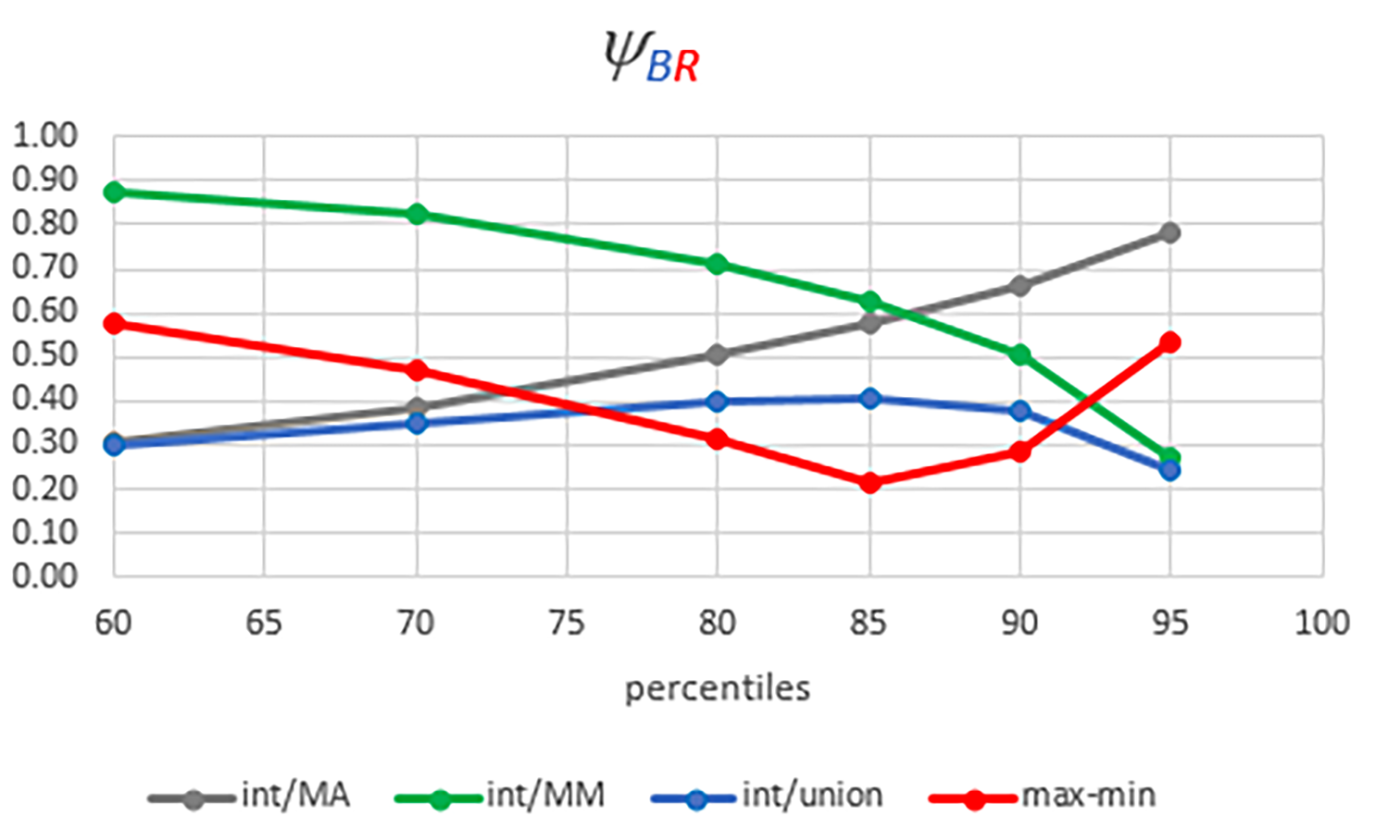
\includegraphics[width=\textwidth]{Imagenes/qibr.png}
         \caption{\textpsi \textsubscript{BR}}
         \label{psiBR}
     \end{subfigure}
     \hfill
     \begin{subfigure}[b]{0.8\textwidth}
         \centering
         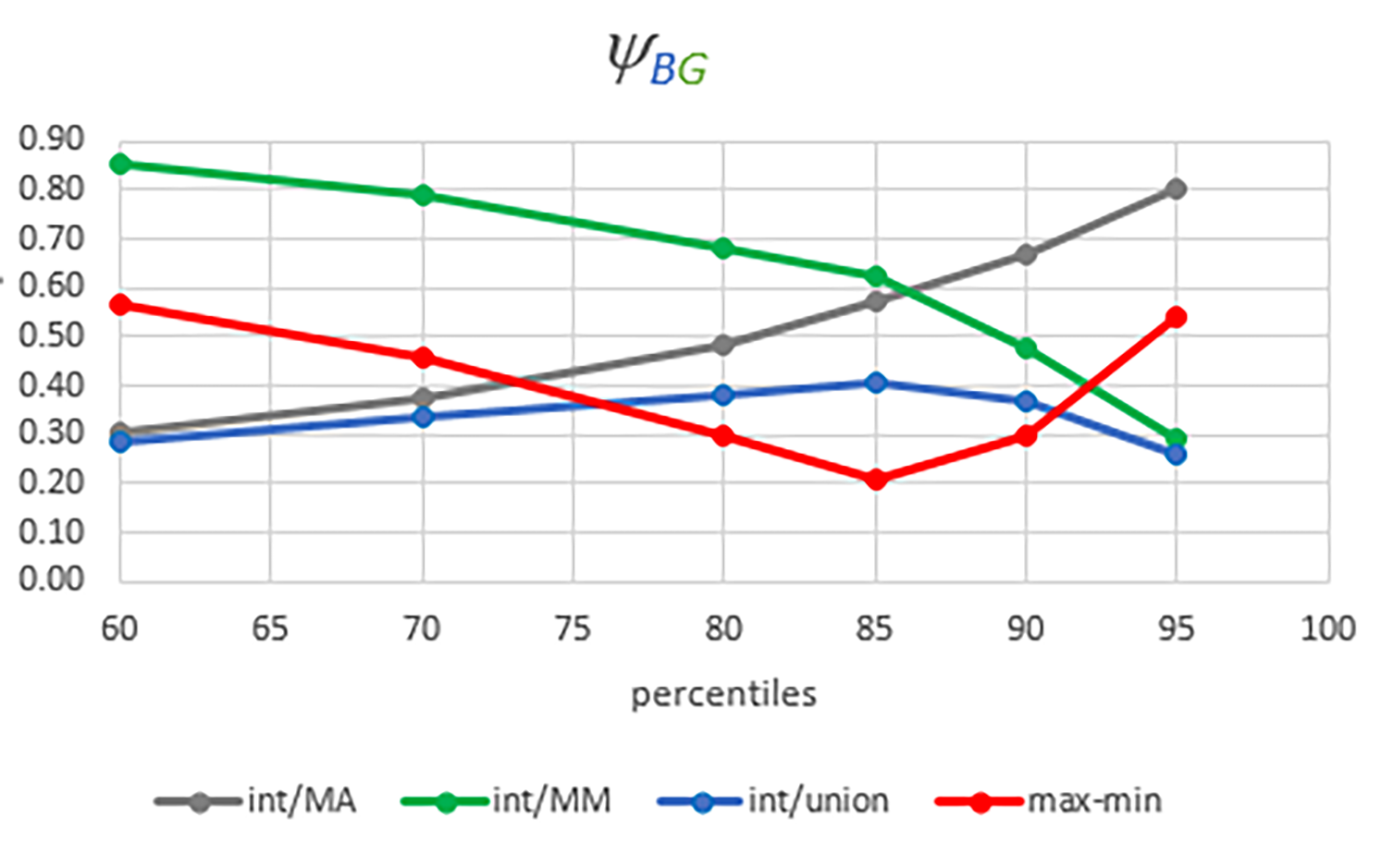
\includegraphics[width=\textwidth]{Imagenes/qibg.png}
         \caption{\textpsi \textsubscript{BG}}
         \label{psiBG}
     \end{subfigure}
     \hfill
     \begin{subfigure}[b]{0.8\textwidth}
         \centering
         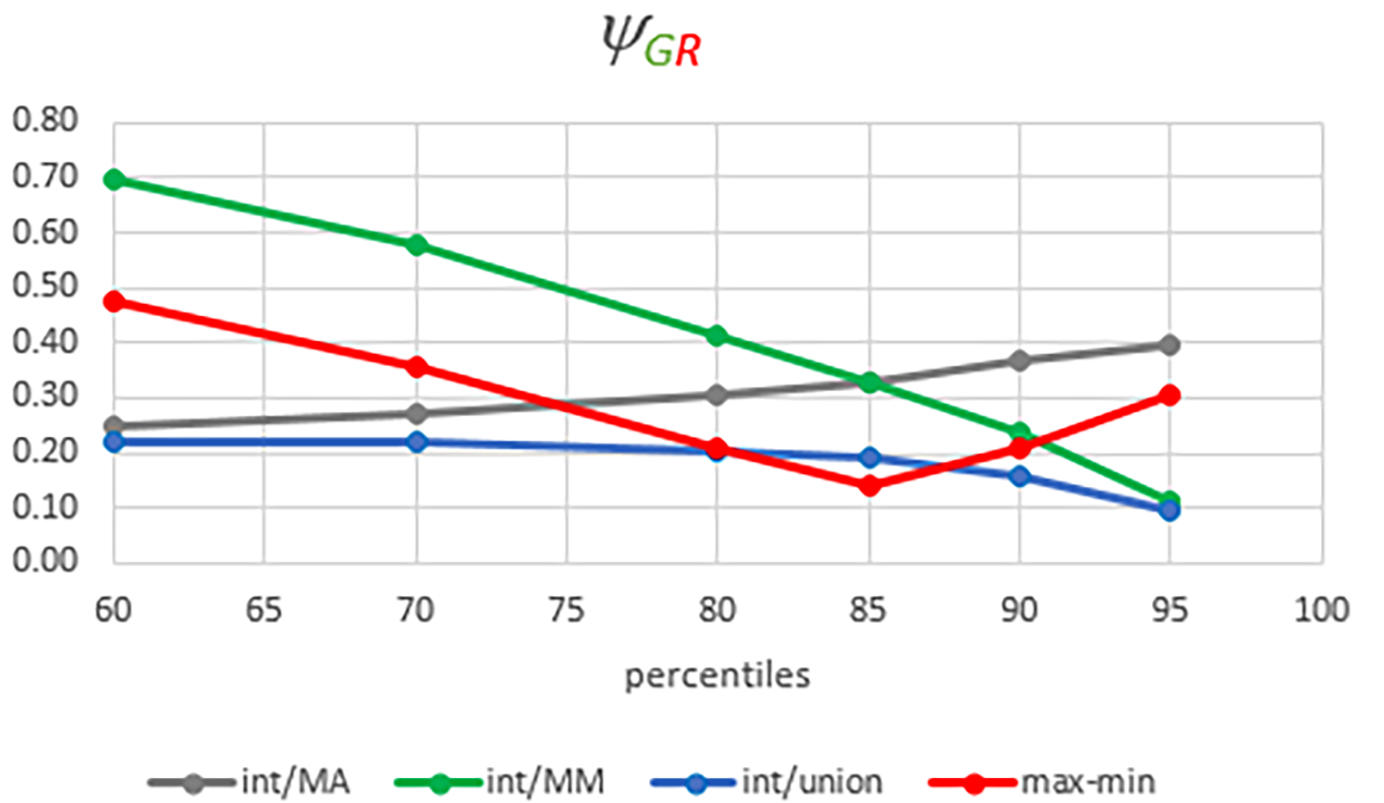
\includegraphics[width=\textwidth]{Imagenes/qigr.png}
         \caption{\textpsi \textsubscript{GR}}
         \label{psiGR}
     \end{subfigure}
        \caption{Índice de calidad}
        \label{quality_index}
\end{figure}

%tamaño
\begin{figure} [h!]
         \centering
         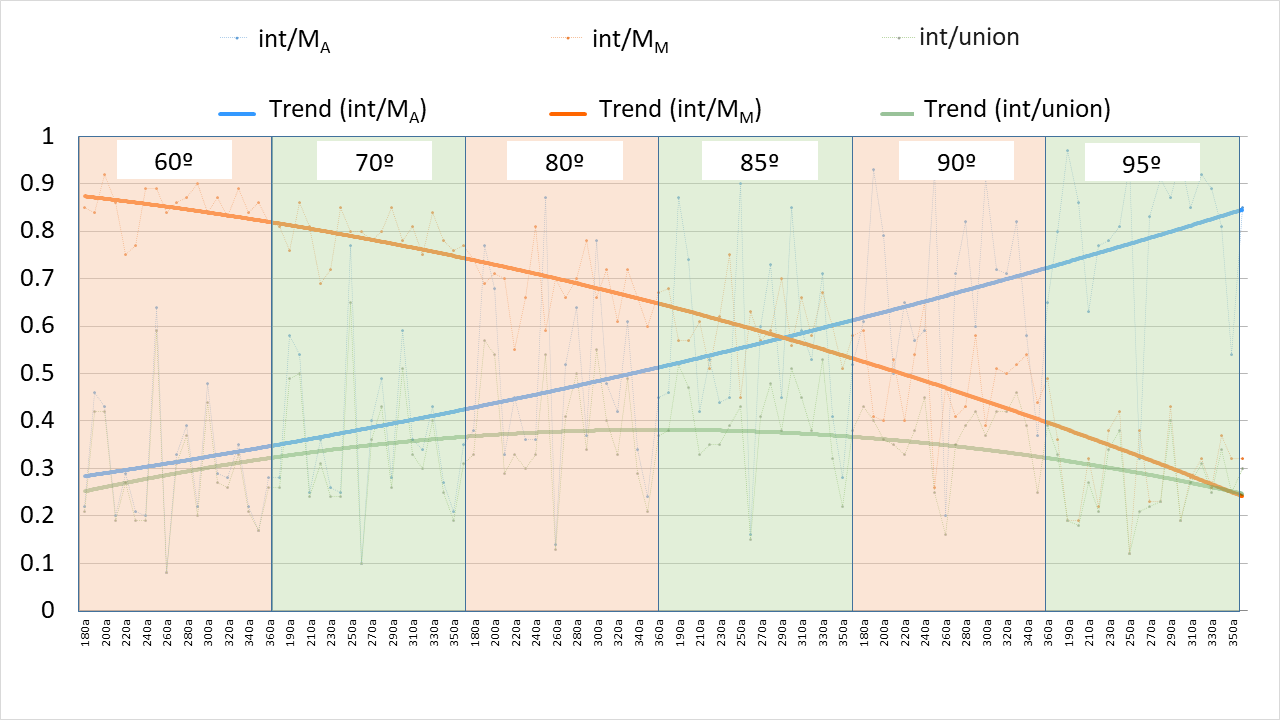
\includegraphics[width=\textwidth]{Imagenes/grafico.png}
         \hfill
         \caption{Curvas índice de calidad}
        \label{curvas_QI}
\end{figure}

%%%%%%%%%%%%%%%%%%%%%%%%%%%%%%%%%%%%%%%%%%%%%%
 


\subsubsection{Validación del método IIC} \label{Validacion}
Superponiendo a una imagen las dos máscaras, una obtenida en forma manual y otra en forma automática, tres expertos realizaron un análisis, calificando el grado de ajuste entre ambas máscaras como <<bueno>>, <<regular>> o <<malo>>. Este procedimiento fue aplicado a cada una de las 19 imágenes analizadas, de modo que se obtuvieron 19 máscaras automáticas por medio del algoritmo para ser comparadas con las respectivas máscaras obtenidas en forma manual. Las superposiciones calificadas como <<buenas>> o <<regulares>> son usadas para seleccionar la mejor máscara automática. Un procedimiento similar se siguió para evaluar el filtrado de la imagen.

\subsubsection{C5-IIC: Análisis de efecto de bandas utilizadas (sombras)} %esto va en capítulo IIC
\paragraph{Informe 1}
A partir de los resultados obtenidos y que se muestran en \ref{Resultados IIC}, se realizaron pruebas del algoritmo sobre distintas imágenes que contienen sombra para ver su desempeño en la selección automática de sombras. En todos los casos el umbral de binarización fue definido considerando el percentil 85 de la distribución de frecuencias del índice invariante de color calculado por la ecuación \ref{invariante de color 1}:
 %%%%%%%%%%%%%%%%%%%%%%%%%%%%%%%%%%%%%% ECUACIÓN %%%%%%%%%%%%%%%%%%%%%%%%%%%%%%%%%%%%%%%%%%%%%%%%%%%%%%%%%
\\
\begin{equation}
	\psi=\frac{4}{\pi} arctan\left(\frac{B\textsubscript{1}-B\textsubscript{2}}{B\textsubscript{1}+B\textsubscript{2}}\right),\label{invariante de color 1}
\end{equation}
\\
%%%%%%%%%%%%%%%%%%%%%%%%%%%%%%%%%%%%%%%%%%%%%%%%%%%%%%%%%%%%%%%%%%%%%%%%%%%%%%%%%%%%%%%%%%%%%%%%%%%%%%%%%
La imagen de la izquierda se procesó con la combinación de las bandas azul y verde ($\Psi_{BG}$), la de la derecha con la combinación azul y rojo ($\Psi_{BR}$).
Se observa que hay mucha similitud en las áreas marcadas, no obstante los diferentes valores de binarización, obtenidos por criterio del 85to percentil de la distribución de frecuencias de los valores de índice invariante de color hallados para cada combinación de bandas.
\\
\\
\paragraph{Informe 2 - }
Aplicando el algoritmo sobre una imagen seleccionada que contiene sombras, usando la ecuación \ref{invariante de color 1} en la combinación de bandas verde y roja y sin utilizar el criterio de percentil para definir el umbral de binarización:

Observando la imagen con la máscara superpuesta en color azul (ver Fig. \ref{Info2}) se nota una marcación altamente coincidente con la que corresponde al área sombreada. Además, mediante el gráfico de histograma de frecuencias del índice invariante de color (Fig. \ref{Info2_histoflor}) es posible advertir el valle entre dos picos situado en torno al valor 0,2 el cual fue usado como umbral de binarización.

\begin{figure}
    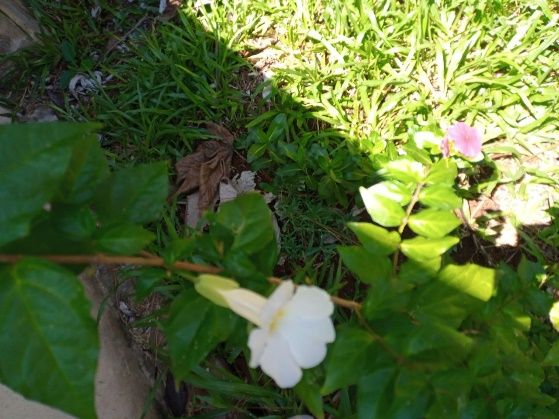
\includegraphics[width=\textwidth]{Imagenes/Informes/info2_flor.jpg}
     \hfill
     \caption{Flor con sombra}
    \label{Info2}
\end{figure}

\begin{figure}
   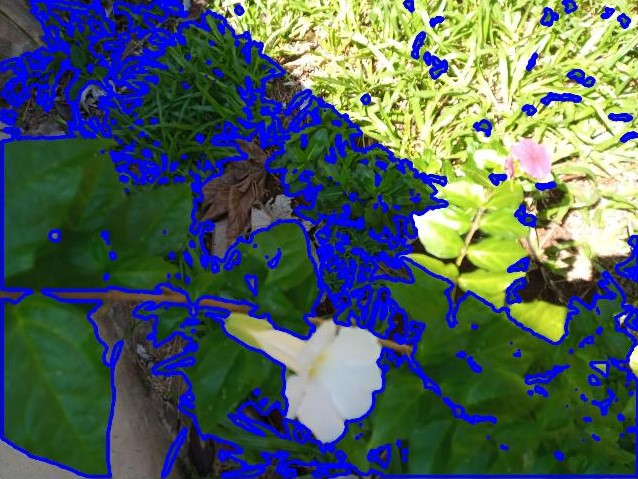
\includegraphics[width=\textwidth]{Imagenes/Informes/info2.jpg}
     \hfill
     \caption{Flor con sombra}
    \label{Info2_flor}
\end{figure}

\begin{figure}
    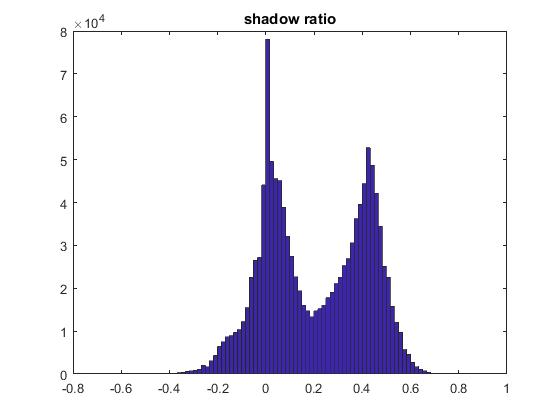
\includegraphics[width=\textwidth]{Imagenes/Informes/info2_histograma.jpg}
     \hfill
     \caption{Histograma}
    \label{Info2_histoflor}
\end{figure} 

\paragraph{Informe 3 - COMBINACIÓN DE BANDAS}

Tal como surge de la ecuación \ref{invariante de color 1}, las posibilidades de combinar dos entre tres bandas de color resultan en seis diferentes índices invariantes de color para una imagen dada. Lo que resulta notorio es que a priori no se sabe cuál de esas seis resulta la más adecuada para constituir la máscara de selección automática de sombras. 

\begin{figure}[H]
    \centering
    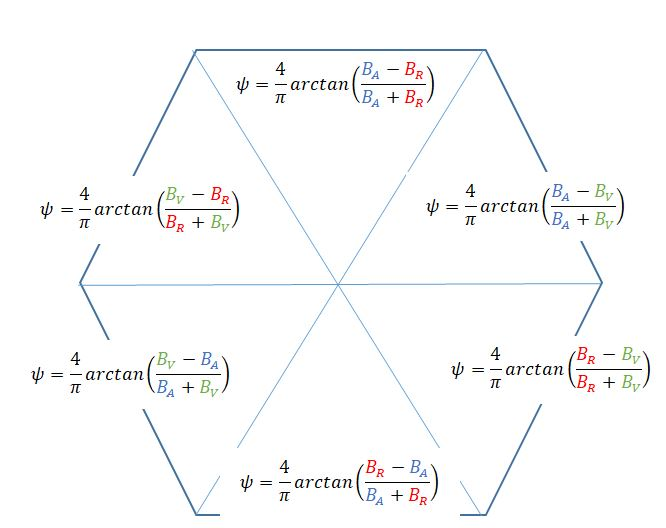
\includegraphics[width=0.5\linewidth]{Imagenes//Comparativo Homo-IIC/hexagono.JPG}
    \caption{Hexágono de posibles combinaciones de la ecuación \ref{invariante de color 1}}
    \label{hexagono}
\end{figure}

Luego de observar las matrices resultantes de aplicar cada una de las seis variantes del índice invariante de color, se evidencia cuál es para el caso dado la combinación más adecuada:

Las combinaciones que mejor evidencian las sombras son BE, RA y RV, y al menos parcialmente, AV, lo que sugeriría la necesidad de recurrir al uso de más de una de ellas para seleccionar las sombras.

Para este caso hay varias posibles combinaciones que evidencian sombra (AV, VA, RA); la RV es mucho más sutil.

En este caso parece preponderar la combinación VERDE menos ROJO (RV)

La presencia de sombras está mejor evidenciada con la combinación VA; RA y RV en forma más sutil

Figuras

\paragraph{Informe 4 - INVARIANTE A RESOLUCIÓN ESPACIAL}
 Según lo que se desprende de una serie de pruebas del algoritmo sobre distintas imágenes, puede observarse que la incidencia del tamaño de la imagen, vale decir, la resolución de la misma, es prácticamente insignificante. Para una misma imagen representada en mayor o menor resolución, las correspondientes máscaras binarias resultantes serán muy semejantes entre sí, como puede comprobarse a la vista:

Figuras

\paragraph{Informe 5 - IMPLEMENTACIÓN DE ALGORITMO EN DIFERENTES PLATAFORMAS}
Se probó implementar el algoritmo en diferentes plataformas, tanto en Matlab y Octave que comparten las líneas de código en los scripts, y también se adaptó para ser ejecutado en R. Asimismo se hizo una prueba usando una planilla de cálculo y por último se usó un programa GIS que permite el cálculo de capas ráster. En todos ellos se pudo obtener a la salida una máscara binaria que corresponde con las áreas sombreadas de la imagen. En el caso de la prueba realizada con la planilla de cálculo se observa que resulta una tarea muy pesada para el programa, ya que este no está optimizado para procesar imágenes. Por tal motivo a los efectos de comparar, se usó un tamaño de imagen reducido, de 400 x 225 píxeles para todos los casos.


Figuras

 
Como puede apreciarse, en los cinco casos las máscaras obtenidas son muy similares. El tamaño de archivos que se generan con el procesamiento en hojas de cálculo hace que sea una opción menos atractiva para este tipo de tareas. Pero queda visto que igualmente puede implementarse.

\paragraph{Informe 6 - TIEMPO DE EJECUCIÓN DEL ALGORITMO EN DIFERENTES PLATAFORMAS}
Se hicieron algunas pruebas para evaluar el tiempo que lleva la ejecución del algoritmo, probando en diferentes plataformas, Matlab, Octave, R. Las pruebas se hicieron con imágenes en distintos tamaños (resoluciones), de 500 x 281 píxeles, 1000 x 562, 2000 x 1125, 4000 x 2250 y 8000 x 4500. Para esa última se simuló una resolución, ya que originalmente las imágenes del dron tienen una resolución de 4000 x 2250 píxeles. Las pruebas que se corrieron en las plataformas Matlab y Octave no difirieron demasiado en el tiempo, que prácticamente ha sido similar en todos los casos, con un tiempo de alrededor de 15 segundos para la imagen de 8000 x 4500 px en Matlab, y 22 segundos en Octave. En cambio fue notorio el incremento de tiempo de ejecución para el caso en R, para la imagen de 4000 x 2250 px llevó alrededor de 17 segundos, y la de 8000 x 4500 px fue imposible determinar el tiempo, ya que desbordó la memoria RAM utilizada. La proporción del incremento del tiempo de ejecución en relación al tamaño de la imagen es de alrededor de tres veces por cada cuadruplicación en tamaño de imagen.


\paragraph{Informe 7 - MOMENTO DE LA CAPTURA}
Para evaluar la incidencia del momento de captura de la imagen aérea en el valor de umbral seleccionado para obtener la máscara binaria de sombras, se comparan dos imágenes de la misma escena capturadas en momentos diferentes, uno alrededor de las ocho de la mañana y otro alrededor de las cuatro de la tarde en una jornada de fines del mes de julio. Procesando las imágenes con el algoritmo y probando diferentes valores de percentil (60, 70, 80, 85, 90 y 95 %)



percentil 60	percentil 70



percentil 80	percentil 85



percentil 90	percentil 95



\color{black}
%%%%%%%%%%%%%%%%%%%%%%%%%%%%%%%%%%%%%%%%%%%%%%%%%%%%%%%%%%%%%%%%%%%%%%%%%%%%%%%%%%%%%%%%%%%%%%%%%%%%%%%%%%%%%%%%%%%%%%%%%%%%%%


\subsection{COMPARACIÓN ENTRE ALGORITMOS}
Tal como puede observarse en las figuras \ref{180_fzz}, \ref{180_eq_fzz}, \ref{180_iic} y \ref{180_eq_iic}, es destacable la robustez del algoritmo de procesamiento por IIC frente al homomórfico. 
\begin{figure}
    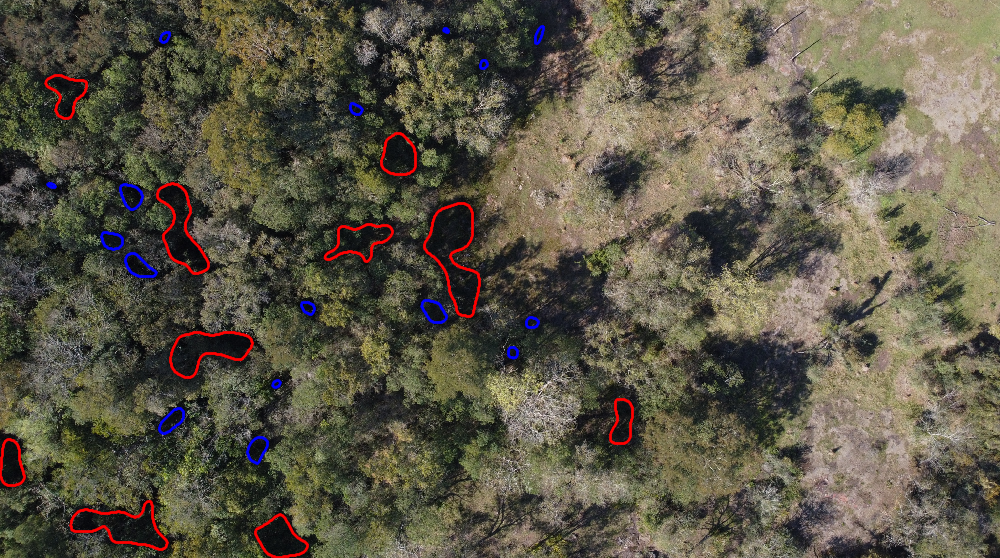
\includegraphics[width=\textwidth]{Imagenes/Comparativo Homo-IIC/180_fzz.png}
     \hfill
     \caption{Selección de sombras llevada a cabo mediante algoritmo de procesamiento homomórfico y posterior inferencia difusa}
    \label{180_fzz}
\end{figure}
\begin{figure}
    \includegraphics[width=\textwidth]{Imagenes/Comparativo Homo-IIC/180_eq_fzz.png}
     \hfill
     \caption{Selección de sombras llevada a cabo mediante algoritmo de procesamiento homomórfico y posterior inferencia difusa, en imagen previamente ecualizada}
    \label{180_eq_fzz}
\end{figure}

\begin{figure}
    \includegraphics[width=\textwidth]{Imagenes/Comparativo Homo-IIC/180_IIC.png}
     \hfill
     \caption{Selección de sombras llevada a cabo mediante algoritmo de procesamiento por índice invariante de color}
    \label{180_iic}
\end{figure}
\begin{figure}
    \includegraphics[width=\textwidth]{Imagenes/Comparativo Homo-IIC/180_eq_IIC.png}
     \hfill
     \caption{Selección de sombras llevada a cabo mediante algoritmo de procesamiento por índice invariante de color, en imagen previamente ecualizada}
    \label{180_eq_iic}
\end{figure}
Correspondiendo las imágenes a la misma escena pero alterando las condiciones de la misma (en este caso una imagen está sin ecualizar y la otra está ecualizada), si se someten al algoritmo de procesamiento homomórfico las diferencias de los resultados son considerables, mientras que al ejecutarse el algoritmo de IIC sobre las mismas, en los resultados apenas se advierte alguna diferencia.